\clearpage
\section{Results\label{sec:results}}

The likelihood described in ref:likelihood is used to
relate yields, uncertainties. It is constructed using ROOTFIT
~\cite{roofit} and maximized using MINUIT~\cite{James:1975dr}.

\subsection{Standard Model\label{sec:smInterp}}

To test compatiblity with a Standard Model only hypothesis,
the signal term is removed from the likelihood model. The parameter values 
maximizing the likelihood function are listed in 
Tables~\ref{tab:mlParameterValues0b_le3j}--\ref{tab:mlParameterValues2b_ge4j}
found in Appendix~\ref{app:ml-params}. The resulting SM yields
along with the observed data yields are summarized in Tables~\ref{app:ml-yields}. 
The uncertainty on the yields are obtained by constructing a probability density
function (p.d.f) from the maximized likelihood, then generating an
ensemble of peudo-experiments from this p.d.f. and maxmizing the same 
likelihood form for each pseudo-experiment, resulting in an esemble of yields.
The $68\%$ quantile of each ensemeble defines the quoted uncertainty on the 
corresponding yield.

Figures~\ref{fig:best-fit-le3j0b}--\ref{fig:best-fit-ge4j2b} show
the \scalht-binned observed data yields (black filled circles) and the
SM expectations and uncertainties (dark blue solid line with light
blue bands) as determined by the fit for the hadronic signal region
and the \mj or both (\mj,\gj) control samples, depending on the event
category. The uncertainties in the SM expectations obtained from the 
ensemble of pseudo-experiments reflect the statistical uncertainties in
the considered data samples and the systematic uncertainties
in the transfer factors as discused in section~\ref{sec:bkgd-syst}.
Figures~\ref{fig:best-fit-le3j0b}--\ref{fig:best-fit-ge4j2b} are summarized
in tabular format in Tables~\ref{tab:ensemble-0b le3j}--\ref{tab:ensemble-2b ge4j} 
in appendix~\ref{app:ml-yields} along with observed data yields and the fit 
result for all event categories and both signal region and control sample bins.

For each \nb, \njet category, the goodness-of-fit of the SM-only hypothesis 
is determined by considering simultaneously all \scalht bins entering
the likelihood. The goodness-of-fit described in ~\cite{Cowan:358560} is obtained
by comparing the nominal maximized likelihood value \lk{data}{max} to 
the corresponding ensemble of values, \lk{}{max}. The quantile which \lk{data}{max}
falls in the distributions is interpreted as a p-value.

The p-values obtained, shown in Figure~\ref{fig:fluct} (Top
Left), are found to be uniformly distributed in the range 0.0--1.0,
with the lowest p-value determined to be 0.17.

%The compatibility of the SM expectation and observed event count is
%also evaluated for each of the 75 signal region bins. A profile
%likelihood ratio is used to determine a p-value and the pull per
%signal region bin. Figure~\ref{fig:fluct} shows the pull as a function
%of the signal region bin (Top Right) and the pull (Bottom Left) and
%p-value (Bottom Right) distributions. The pulls appear to be randomly
%distributed across signal region bins with no obvious structure. The
%pull distribution approximates a Gaussian-like behaviour. The
%probability for the observed positive tail in the pull distribution to
%occur by chance is higher than 0.5\%, and there is no excess of
%outliers beyond $2\sigma$. In summary, the observed result is
%consistent with an, albeit rare, statistical fluctuation.
%
\begin{figure}[h!]
  \begin{center}
    \subfigure[p-values per event category.]{
      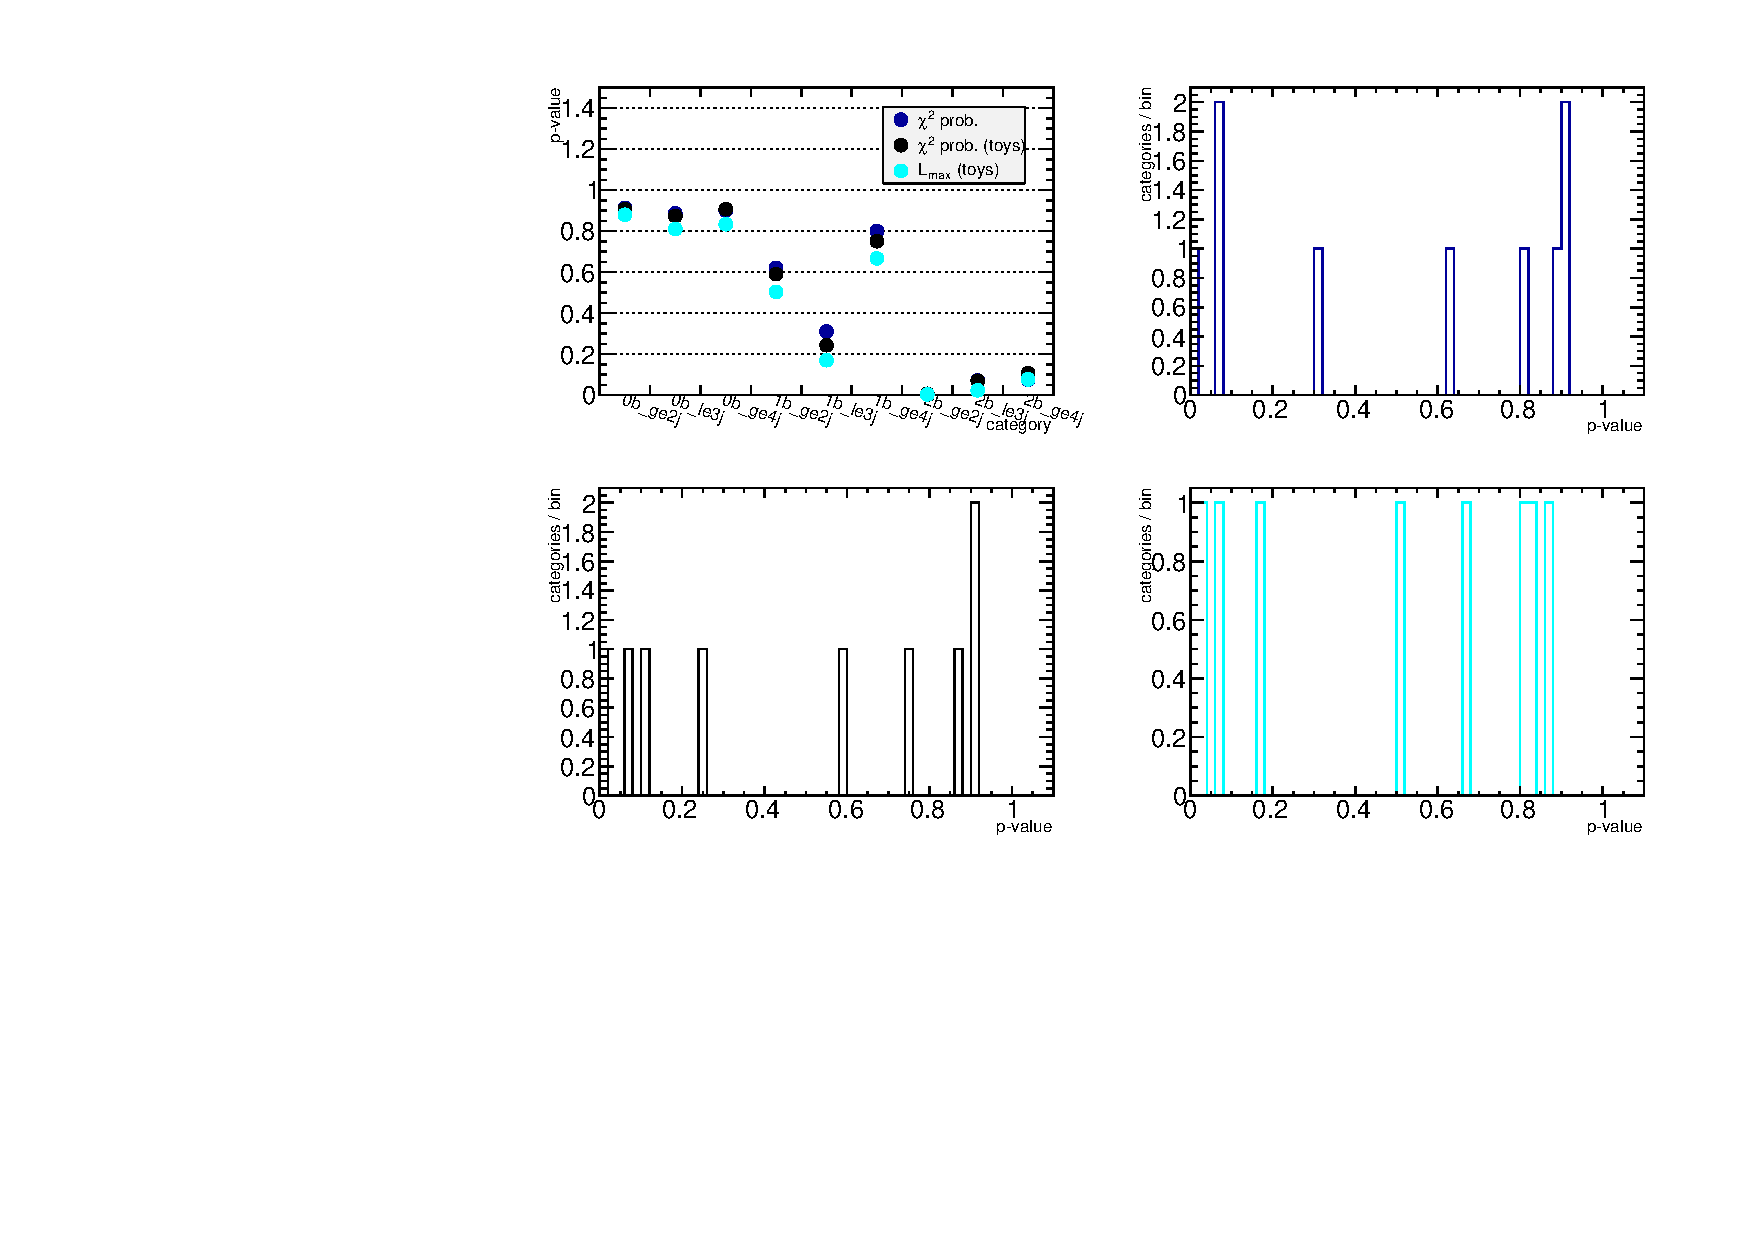
\includegraphics[width=0.45\textwidth, trim=0 190 290 20, clip=true]{figures/fit/v21/pValues} % lbrt
    } 
    \subfigure[Pull versus signal region bin.]{
      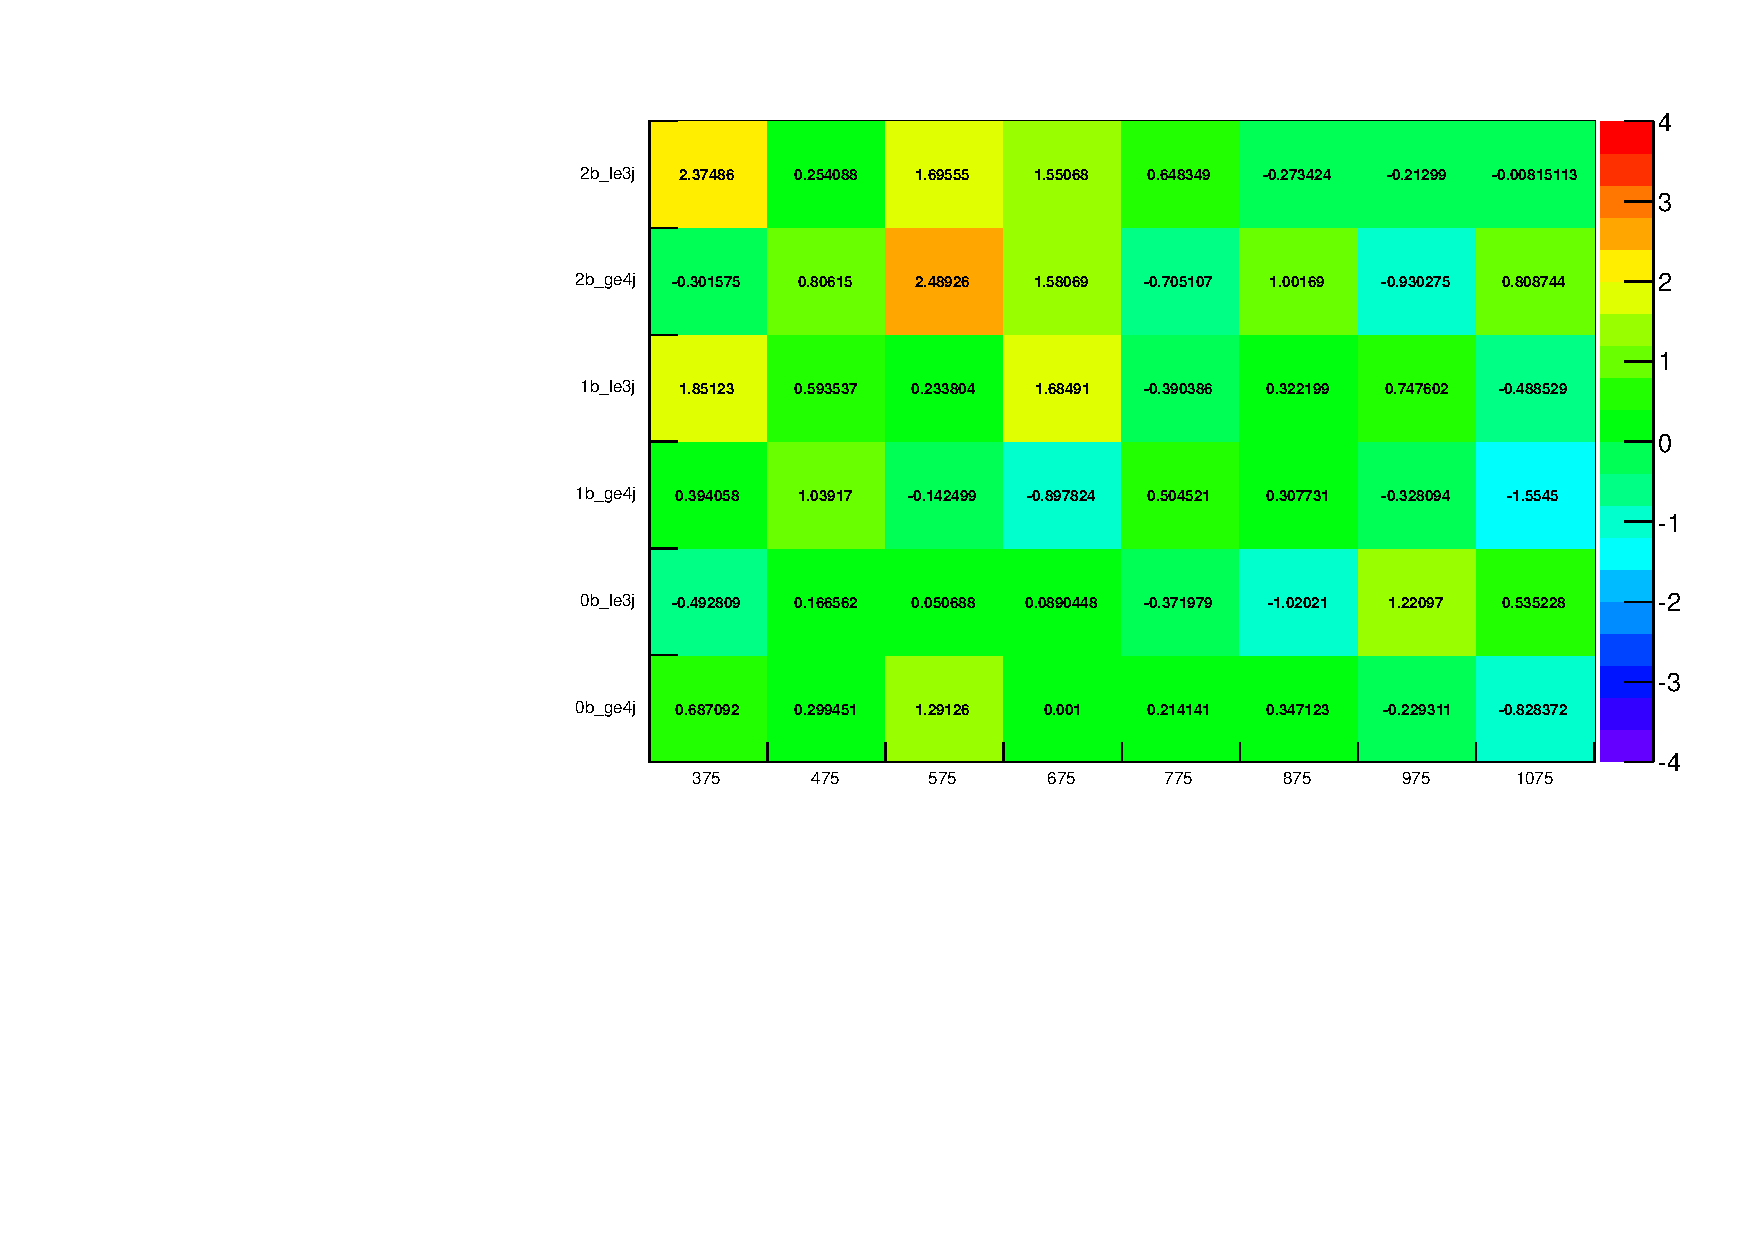
\includegraphics[width=0.45\textwidth, trim=0 0 0 30, clip=true]{figures/fit/v21/significances_catVsHt_wTrig}
    } \\
%    \subfigure[Pull per signal region bin.]{
%      \includegraphics[width=0.45\textwidth, trim=0 0 0 0, clip=true]{figures/fit/v1/pull_per_bin_gaus}
%    } 
%    \subfigure[p-value per signal region bin.]{
%      \includegraphics[width=0.45\textwidth, trim=0 0 0 0, clip=true]{figures/fit/v1/pvalue_per_bin}
%    } \\
    \caption{Pulls and p-values. See text for details}
    \label{fig:fluct}
  \end{center}
\end{figure}

%Figures~\ref{fig:best-fit-control-only-le3j0b}--\ref{fig:best-fit-control-only-ge4jge4b}
%show the observed data yields (black filled circles) and SM
%expectations and associated uncertainties (dark green solid line with
%light green bands). In this case, the hadronic signal region yields
%are not considered and the SM predictions are determined solely from
%the \mj or all three data control samples (depending on the event
%category). Figures~\ref{fig:best-fit-control-only-le3j0b}--\ref{fig:best-fit-control-only-ge4jge4b}
%and Figures~\ref{fig:best-fit-le3j0b}--\ref{fig:best-fit-ge4jge4b}
%correspond to ``a priori'' and ``a posteriori'' fits, respectively.
%In addition, Table~\ref{tab:ensemble-summary-priori} summarises the
%observed data yields and the fit result for all event categories and
%all signal region bins for the ``a priori'' fit.  The uncertainties in
%the SM expectations are smaller for the ``a posteriori'' fit due to
%the additional information from hadronic signal region counts.
%
%\begin{landscape}
\begin{center}
\begin{table}[h!]
  \caption{Summary of hadronic yields from fit.}
  \label{tab:ensemble-summary-posteriori}
  \centering
  \scriptsize
\begin{tabular}{ lllllllll }

\hline
& 375--475                       & 475--575                       & 575--675                       & 675--775                       & 775--875                       & 875--975                       & 975--1075                      & 1075--$\infty$                 \\ [1.000000ex]
\hline
0b le3j SM \T   & $2637^{+50}_{-48}$             & $759^{+24}_{-23}$              & $252^{+14}_{-13}$              & $76.5^{+6.6}_{-4.7}$           & $33.7^{+3.5}_{-3.7}$           & $11.8^{+2.1}_{-2.3}$           & $6.3^{+1.4}_{-1.2}$            & $3.2^{+0.9}_{-0.9}$            \\ 
0b le3j Data \T & $2627$                         & $762$                          & $253$                          & $77$                           & $32$                           & $9$                            & $9$                            & $4$                            \\ 
\hline
1b le3j SM \T   & $413^{+15}_{-14}$              & $111^{+6}_{-4}$                & $35.8^{+3.4}_{-2.7}$           & $10.1^{+1.6}_{-1.3}$           & $3.7^{+0.8}_{-0.8}$            & $1.6^{+0.6}_{-0.7}$            & $0.5^{+0.3}_{-0.4}$            & $0.1^{+0.1}_{-0.0}$            \\ 
1b le3j Data \T & $440$                          & $116$                          & $37$                           & $15$                           & $3$                            & $2$                            & $1$                            & $0$                            \\ 
\hline
2b le3j SM \T   & $63.0^{+3.9}_{-4.1}$           & $18.0^{+1.3}_{-1.4}$           & $4.2^{+0.6}_{-0.5}$            & $1.1^{+0.2}_{-0.2}$            & $0.2^{+0.1}_{-0.1}$            & $0.0^{+0.0}_{-0.0}$            & $0.0^{+0.0}_{-0.0}$            & $0.0^{+0.0}_{-0.0}$            \\ 
2b le3j Data \T & $80$                           & $19$                           & $8$                            & $3$                            & $0$                            & $0$                            & $0$                            & $0$                            \\ 
\hline
0b ge4j SM \T   & $460^{+16}_{-15}$              & $298^{+12}_{-11}$              & $146^{+7}_{-7}$                & $66.0^{+4.4}_{-5.5}$           & $27.1^{+3.2}_{-3.5}$           & $14.0^{+2.0}_{-1.9}$           & $6.5^{+1.4}_{-1.5}$            & $3.2^{+1.0}_{-1.0}$            \\ 
0b ge4j Data \T & $470$                          & $302$                          & $158$                          & $66$                           & $28$                           & $15$                           & $6$                            & $2$                            \\ 
\hline
1b ge4j SM \T   & $192^{+9}_{-8}$                & $122^{+6}_{-6}$                & $44.8^{+3.2}_{-3.7}$           & $17.1^{+2.4}_{-2.0}$           & $6.8^{+1.2}_{-1.3}$            & $5.4^{+1.5}_{-1.5}$            & $2.4^{+1.0}_{-0.8}$            & $1.2^{+0.8}_{-0.8}$            \\ 
1b ge4j Data \T & $196$                          & $132$                          & $44$                           & $14$                           & $8$                            & $6$                            & $2$                            & $0$                            \\ 
\hline
2b ge4j SM \T   & $74.2^{+4.2}_{-4.4}$           & $47.0^{+3.2}_{-3.3}$           & $20.1^{+2.0}_{-1.8}$           & $7.7^{+1.3}_{-1.1}$            & $1.9^{+0.3}_{-0.3}$            & $0.9^{+0.2}_{-0.2}$            & $0.4^{+0.1}_{-0.1}$            & $0.4^{+0.2}_{-0.1}$            \\ 
2b ge4j Data\T & $72$                           & $52$                           & $31$                           & $12$                           & $1$                            & $2$                            & $0$                            & $1$                            \\ 
\hline
  \end{tabular}
\end{table}
\end{center}
%\end{landscape}

%\begin{landscape}
%\begin{center}
%\begin{table}[h!]
%  \caption{Summary of the ``a priori'' fit.}
%  \label{tab:ensemble-summary-priori}
%  \centering
%  \scriptsize
%  \begin{tabular}{ llllllllllllll }
%    \hline
%    \hline
%    \multicolumn{2}{c}{} & \multicolumn{11}{c}{\scalht (GeV)}                                                                                                                                                                                                                                              \\ 
%    \njet                & \nb      &        & 200--275              & 275--325             & 325--375              & 375--475             & 475--575              & 575--675             & 675--775             & 775--875             & 875--975             & 975--1075           & 1075--$\infty$      \\ 
%    \hline
%    2--3                 & $0$      & SM\T   & $12391^{+368}_{-325}$ & $5566^{+325}_{-188}$ & $3424^{+205}_{-149}$  & $2473^{+131}_{-96}$  & $684^{+38}_{-34}$     & $231^{+18}_{-19}$    & $69.8^{+6.1}_{-6.6}$ & $27.9^{+3.9}_{-3.2}$ & $11.0^{+2.1}_{-1.8}$ & $5.4^{+0.8}_{-1.0}$ & $3.7^{+0.9}_{-0.8}$ \\ 
%    2--3                 & $0$      & Data\T & $13310$               & $5404$               & $3580$                & $2475$               & $698$                 & $224$                & $81$                 & $28$                 & $12$                 & $9$                 & $3$                 \\ 
%    2--3                 & $1$      & SM\T   & $1626^{+60}_{-47}$    & $862^{+48}_{-41}$    & $548^{+29}_{-35}$     & $413^{+28}_{-23}$    & $103^{+8}_{-7}$       & $26.6^{+3.1}_{-3.2}$ & $9.5^{+1.2}_{-1.6}$  & $3.1^{+0.9}_{-0.8}$  & $2.6^{+0.9}_{-0.8}$  & $0.4^{+0.2}_{-0.2}$ & $0.2^{+0.1}_{-0.1}$ \\ 
%    2--3                 & $1$      & Data\T & $1802$                & $835$                & $597$                 & $416$                & $97$                  & $29$                 & $7$                  & $4$                  & $1$                  & $0$                 & $0$                 \\ 
%    2--3                 & $2$      & SM\T   & $177^{+9}_{-7}$       & $113^{+7}_{-7}$      & $97.3^{+6.3}_{-6.6}$  & $66.0^{+6.3}_{-5.8}$ & $14.6^{+1.7}_{-1.4}$  & $2.9^{+0.5}_{-0.5}$  & $1.1^{+0.2}_{-0.3}$  & $0.2^{+0.1}_{-0.1}$  & $0.1^{+0.1}_{-0.0}$  & \multicolumn{2}{c}{}                      \\ 
%    2--3                 & $2$      & Data\T & $174$                 & $119$                & $117$                 & $70$                 & $18$                  & $7$                  & $1$                  & $0$                  & $0$                  & \multicolumn{2}{c}{}                      \\ 
%    $\geq 4$             & $0$      & SM\T   & $106^{+10}_{-10}$     & $520^{+32}_{-34}$    & $448^{+39}_{-54}$     & $369^{+31}_{-25}$    & $224^{+17}_{-15}$     & $109^{+14}_{-13}$    & $46.8^{+5.8}_{-6.1}$ & $19.2^{+2.8}_{-2.7}$ & $9.2^{+1.7}_{-1.7}$  & $3.7^{+1.1}_{-0.9}$ & $3.2^{+0.7}_{-0.7}$ \\ 
%    $\geq 4$             & $0$      & Data\T & $103$                 & $590$                & $455$                 & $391$                & $274$                 & $149$                & $56$                 & $18$                 & $12$                 & $7$                 & $8$                 \\ 
%    $\geq 4$             & $1$      & SM\T   & $39.8^{+3.2}_{-3.5}$  & $223^{+14}_{-12}$    & $211^{+25}_{-23}$     & $171^{+18}_{-15}$    & $98.7^{+10.1}_{-9.1}$ & $35.5^{+6.0}_{-5.1}$ & $14.8^{+2.2}_{-2.2}$ & $6.8^{+1.5}_{-1.2}$  & $3.2^{+0.9}_{-0.9}$  & $1.1^{+0.5}_{-0.4}$ & $1.2^{+0.4}_{-0.4}$ \\ 
%    $\geq 4$             & $1$      & Data\T & $38$                  & $207$                & $250$                 & $181$                & $108$                 & $41$                 & $10$                 & $14$                 & $6$                  & $1$                 & $1$                 \\ 
%    $\geq 4$             & $2$      & SM\T   & $13.0^{+1.0}_{-0.9}$  & $75.5^{+4.8}_{-4.8}$ & $96.1^{+11.4}_{-9.4}$ & $69.5^{+7.2}_{-8.3}$ & $43.9^{+4.8}_{-5.7}$  & $16.1^{+3.7}_{-2.7}$ & $5.2^{+1.2}_{-0.9}$  & $1.7^{+0.3}_{-0.4}$  & $1.9^{+0.5}_{-0.4}$  & \multicolumn{2}{c}{}                      \\ 
%    $\geq 4$             & $2$      & Data\T & $17$                  & $82$                 & $95$                  & $86$                 & $48$                  & $19$                 & $10$                 & $2$                  & $1$                  & \multicolumn{2}{c}{}                      \\ 
%    $\geq 4$             & $3$      & SM\T   & $1.0^{+0.2}_{-0.2}$   & $8.1^{+0.8}_{-0.8}$  & $11.7^{+1.9}_{-1.6}$  & $8.0^{+1.4}_{-1.2}$  & $5.3^{+1.2}_{-0.8}$   & $2.3^{+0.6}_{-0.5}$  & $0.8^{+0.2}_{-0.2}$  & $0.2^{+0.1}_{-0.1}$  & $0.2^{+0.1}_{-0.1}$  & \multicolumn{2}{c}{}                      \\ 
%    $\geq 4$             & $3$      & Data\T & $0$                   & $9$                  & $8$                   & $8$                  & $9$                   & $1$                  & $3$                  & $0$                  & $0$                  & \multicolumn{2}{c}{}                      \\ 
%    $\geq 4$             & $\geq 4$ & SM\T   & $0.0^{+0.0}_{-0.0}$  & $0.1^{+0.1}_{-0.1}$  & $0.6^{+0.3}_{-0.3}$   & $0.7^{+0.3}_{-0.3}$  & \multicolumn{7}{l}{}                                                                                                                                          \\ 
%    $\geq 4$             & $\geq 4$ & Data\T & $0$                   & $0$                  & $0$                   & $3$                  & \multicolumn{7}{l}{}                                                                                                                                          \\ 
%    \hline
%    \hline
%  \end{tabular}
%\end{table}
%\end{center}
%\end{landscape}
%
\clearpage
\begin{figure}[t!]
  \begin{center}
    \subfigure[Hadronic sample (linear scale)]{
      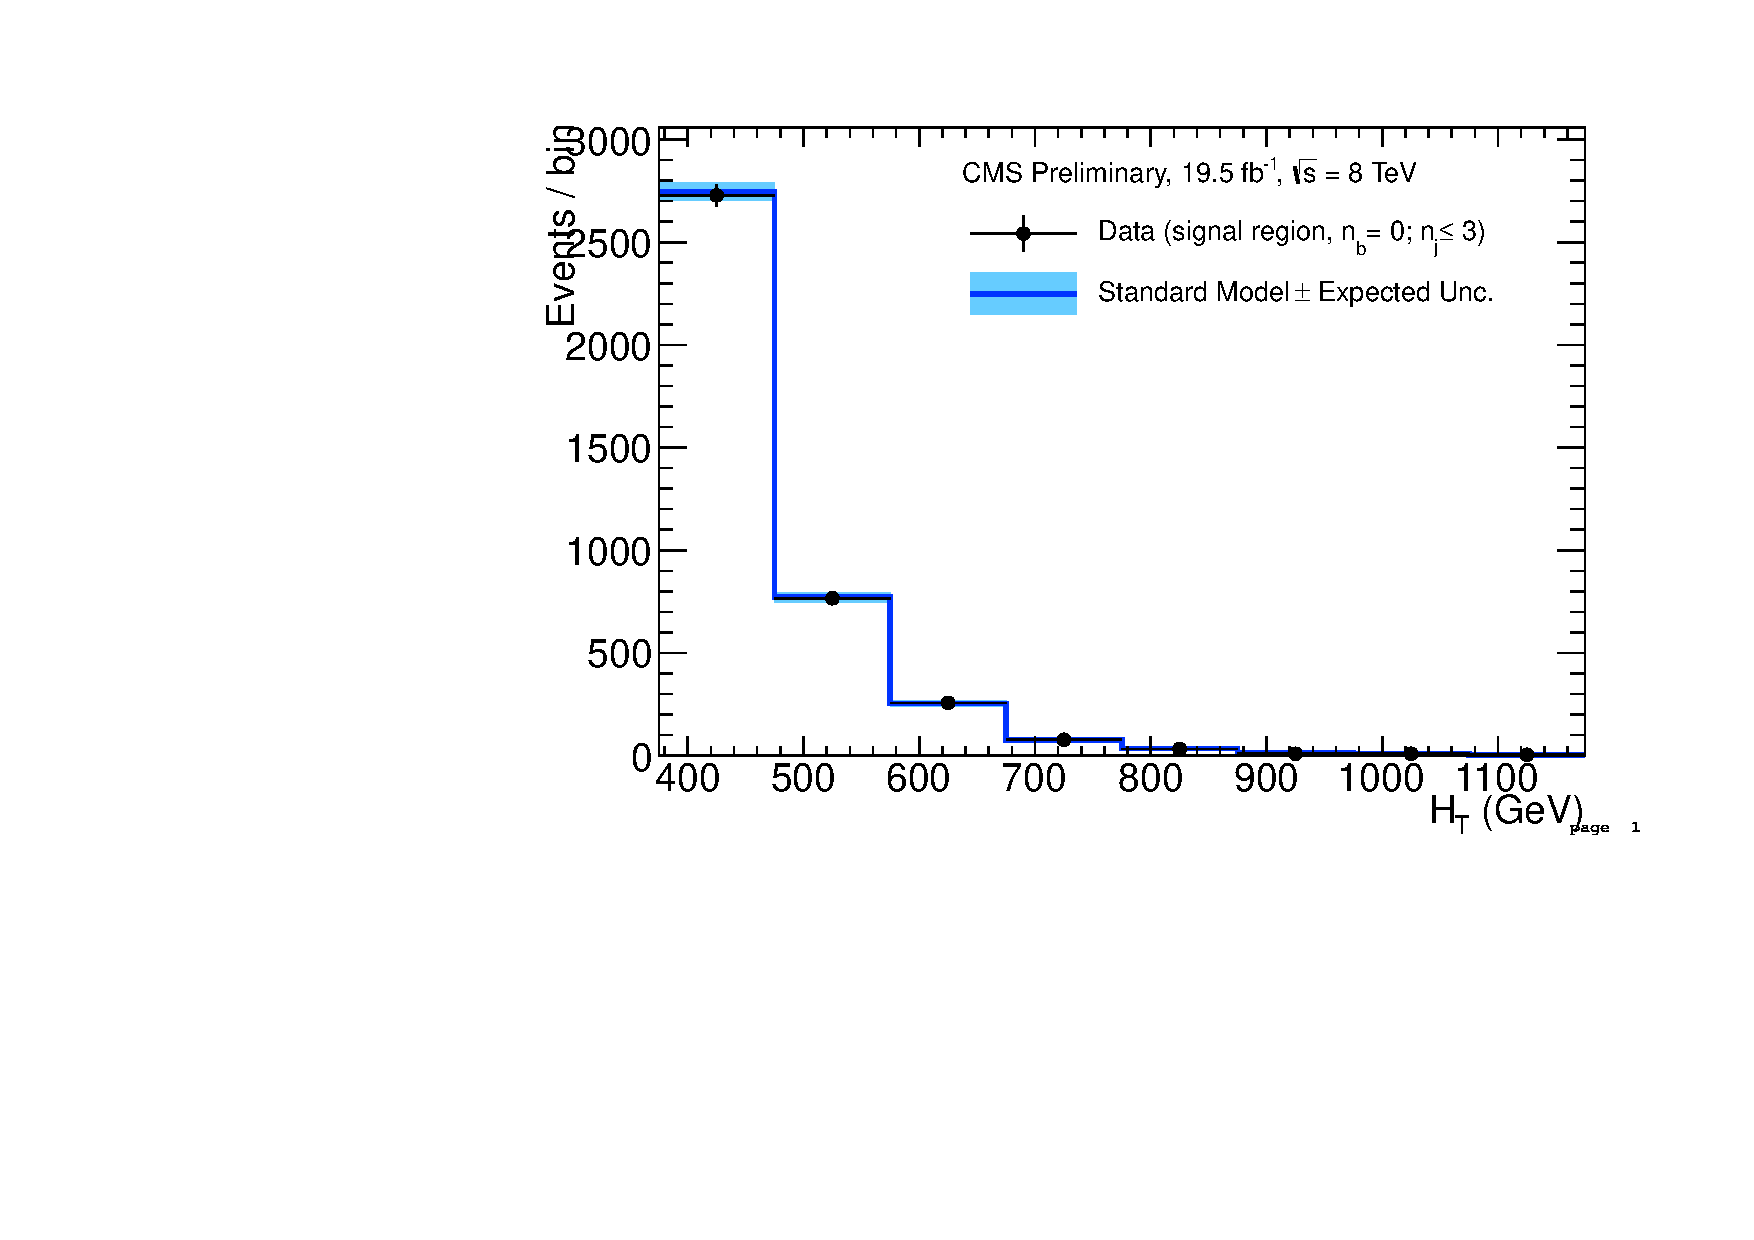
\includegraphics[width=0.45\textwidth,page=1]{figures/fit/v22/bestFit_2012pf_RQcdZero_fZinvAll_0b_le3j-1hp_smOnly}
    } 
    \subfigure[Hadronic sample (logarithmic scale)]{
      \includegraphics[width=0.45\textwidth,page=2]{figures/fit/v22/bestFit_2012pf_RQcdZero_fZinvAll_0b_le3j-1hp_smOnly}
    } \\
    \subfigure[$\mu$ + jets sample]{
      \includegraphics[width=0.45\textwidth,page=4]{figures/fit/v22/bestFit_2012pf_RQcdZero_fZinvAll_0b_le3j-1hp_smOnly}
    } 
    \subfigure[$\gamma$ + jets sample]{
      \includegraphics[width=0.45\textwidth,page=6]{figures/fit/v22/bestFit_2012pf_RQcdZero_fZinvAll_0b_le3j-1hp_smOnly}
    } 
    \caption{\label{fig:best-fit-le3j0b} Comparison of the
      \scalht-binned observed data yields and SM expectations when
      requiring \njetlow and $\nb = 0$ for the (a-b) hadronic, (c)
      \mj, (d) \mmj and (e) \gj samples, as determined by a
      simultaneous fit to all data samples under the SM-only
      hypothesis. The observed event yields in data (black dots) and
      the expectations and their uncertainties (dark blue solid line
      with light blue bands), as determined by the simultaneous fit,
      are shown. %For illustrative purposes only, the signal
      %expectations (pink dashed line) for the model \texttt{T2cc} with
      %$m_{\sq} = 250\GeV$ and $m_{\text{LSP}} = 240\GeV$ are stacked
      %on top of the SM expectations.
      }
  \end{center}
\end{figure}

\clearpage
\begin{figure}[t!]
  \begin{center}
    \subfigure[Hadronic sample (linear scale)]{
      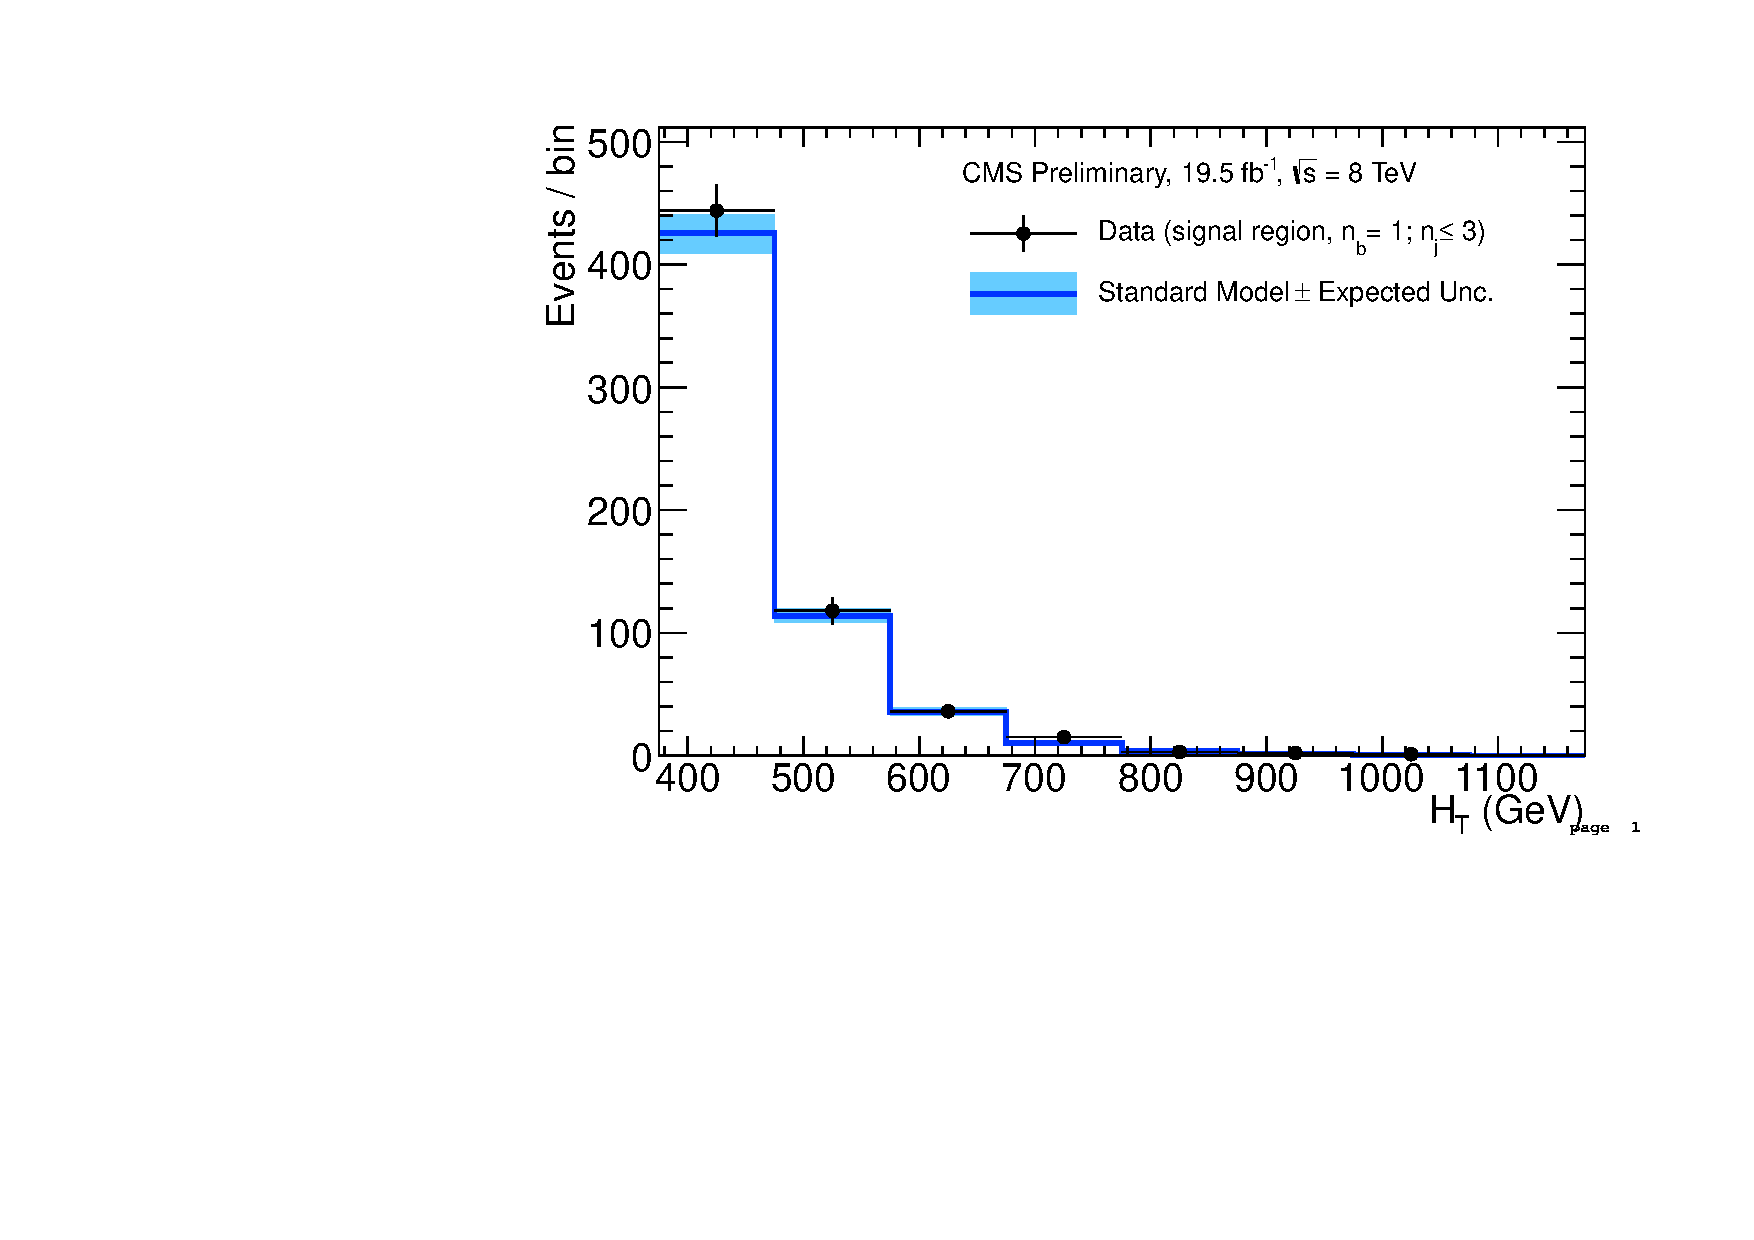
\includegraphics[width=0.45\textwidth,page=1]{figures/fit/v22/bestFit_2012pf_RQcdZero_fZinvAll_1b_le3j-1hp_smOnly}
    } 
    \subfigure[Hadronic sample (logarithmic scale)]{
      \includegraphics[width=0.45\textwidth,page=2]{figures/fit/v22/bestFit_2012pf_RQcdZero_fZinvAll_1b_le3j-1hp_smOnly}
    } \\
    \subfigure[$\mu$ + jets sample]{
      \includegraphics[width=0.45\textwidth,page=4]{figures/fit/v22/bestFit_2012pf_RQcdZero_fZinvAll_1b_le3j-1hp_smOnly}
    } 
    \subfigure[$\gamma$ + jets sample]{
      \includegraphics[width=0.45\textwidth,page=6]{figures/fit/v22/bestFit_2012pf_RQcdZero_fZinvAll_1b_le3j-1hp_smOnly}
    } 
    \caption{\label{fig:best-fit-le3j1b} Comparison of the
      \scalht-binned observed data yields and SM expectations when
      requiring \njetlow and $\nb = 1$ for the (a-b) hadronic, (c)
      \mj, (d) \mmj and (e) \gj samples, as determined by a
      simultaneous fit to all data samples under the SM-only
      hypothesis. The observed event yields in data (black dots) and
      the expectations and their uncertainties (dark blue solid line
      with light blue bands), as determined by the simultaneous fit,
      are shown. %For illustrative purposes only, the signal
      %expectations (pink dashed line) for the model \texttt{T2cc} with
      %$m_{\sq} = 250\GeV$ and $m_{\text{LSP}} = 170\GeV$ are stacked
      %on top of the SM expectations.
      }
  \end{center}
\end{figure}

\clearpage
\begin{figure}[t!]
  \begin{center}
    \subfigure[Hadronic sample (linear scale)]{
      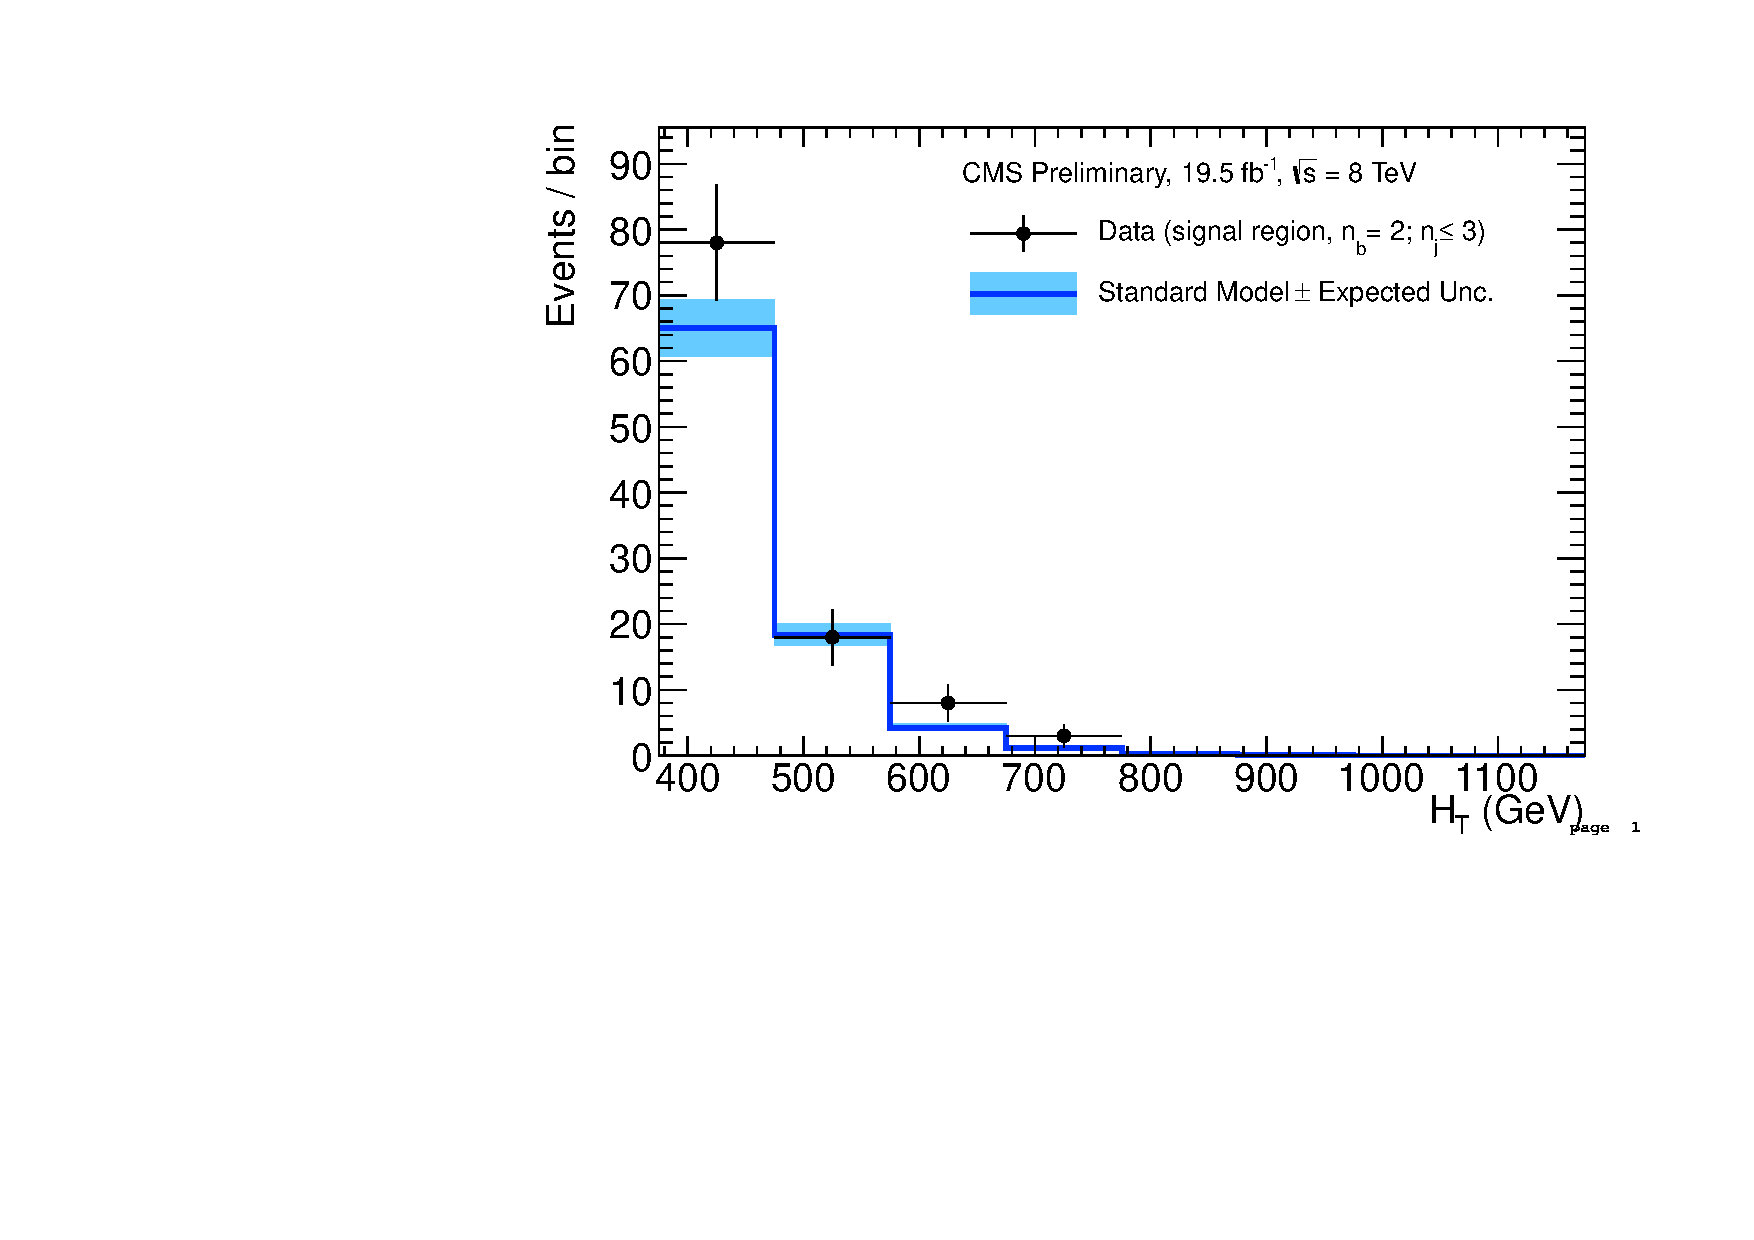
\includegraphics[width=0.45\textwidth,page=1]{figures/fit/v22/bestFit_2012pf_RQcdZero_fZinvAll_2b_le3j-1h_smOnly}
    } 
    \subfigure[Hadronic sample (logarithmic scale)]{
      \includegraphics[width=0.45\textwidth,page=2]{figures/fit/v22/bestFit_2012pf_RQcdZero_fZinvAll_2b_le3j-1h_smOnly}
    } \\
    \subfigure[$\mu$ + jets sample]{
      \includegraphics[width=0.45\textwidth,page=4]{figures/fit/v22/bestFit_2012pf_RQcdZero_fZinvAll_2b_le3j-1h_smOnly}
    } 
    \caption{\label{fig:best-fit-le3j2b} Comparison of the
      \scalht-binned observed data yields and SM expectations when
      requiring \njetlow and $\nb = 2$ for the (a-b) hadronic and \mj
      samples, as determined by a simultaneous fit to both the
      hadronic and \mj data samples under the SM-only hypothesis. The
      observed event yields in data (black dots) and the expectations
      and their uncertainties (dark blue solid line with light blue
      bands), as determined by the simultaneous fit, are shown. }
%      For illustrative purposes only, the signal expectations (pink
%      dashed line) for the model \texttt{T2cc} with $m_{\sq} =
%      250\GeV$ and $m_{\text{LSP}} = 240\GeV$ are stacked on top of
%      the SM expectations.}
  \end{center}
\end{figure}

\clearpage
\begin{figure}[t!]
  \begin{center}
    \subfigure[Hadronic sample (linear scale)]{
      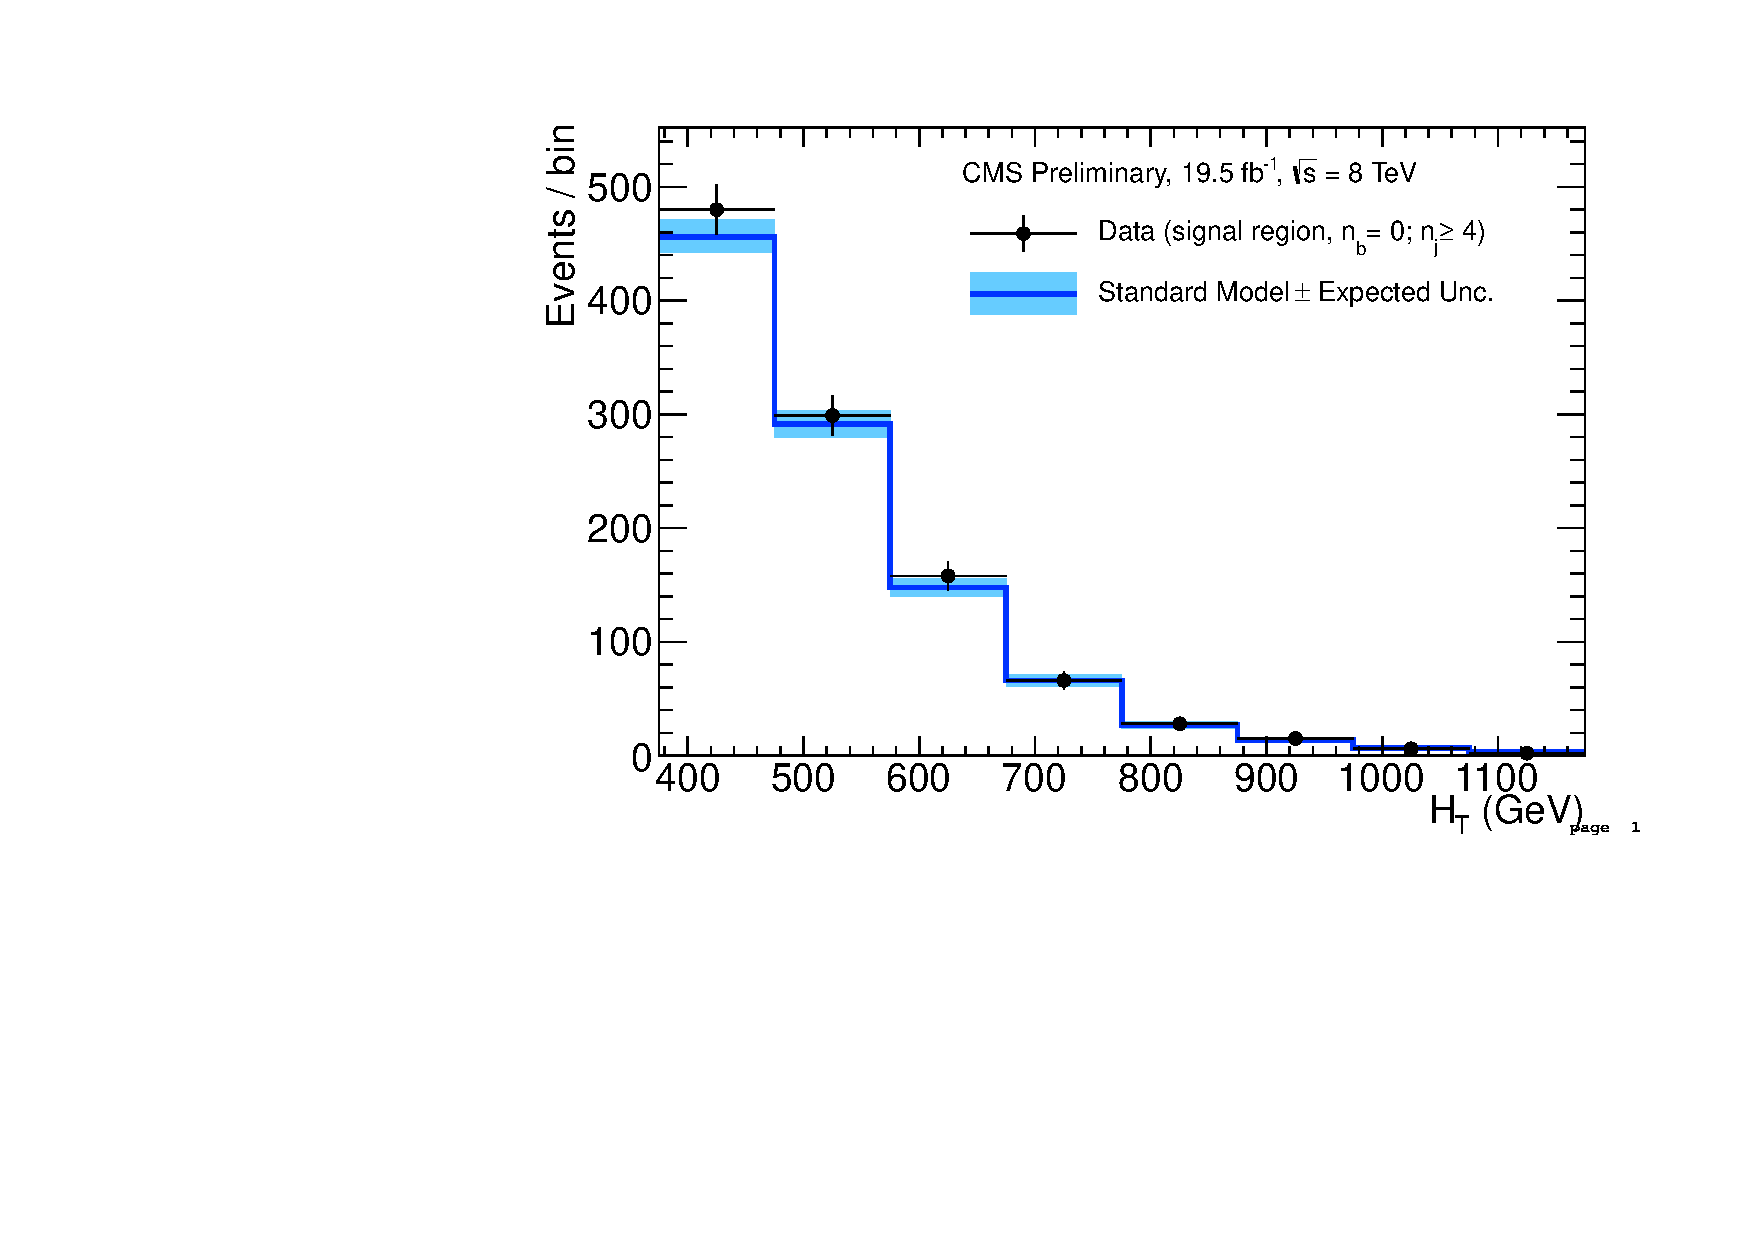
\includegraphics[width=0.45\textwidth,page=1]{figures/fit/v22/bestFit_2012pf_RQcdZero_fZinvAll_0b_ge4j-1hp_smOnly}
    } 
    \subfigure[Hadronic sample (logarithmic scale)]{
      \includegraphics[width=0.45\textwidth,page=2]{figures/fit/v22/bestFit_2012pf_RQcdZero_fZinvAll_0b_ge4j-1hp_smOnly}
    } \\
    \subfigure[$\mu$ + jets sample]{
      \includegraphics[width=0.45\textwidth,page=4]{figures/fit/v22/bestFit_2012pf_RQcdZero_fZinvAll_0b_ge4j-1hp_smOnly}
    } 
    \subfigure[$\gamma$ + jets sample]{
      \includegraphics[width=0.45\textwidth,page=6]{figures/fit/v22/bestFit_2012pf_RQcdZero_fZinvAll_0b_ge4j-1hp_smOnly}
    } 
    \caption{\label{fig:best-fit-ge4j0b} Comparison of the
      \scalht-binned observed data yields and SM expectations when
      requiring \njethigh and $\nb = 0$ for the (a-b) hadronic, (c)
      \mj, (d) \mmj and (e) \gj samples, as determined by a
      simultaneous fit to all data samples under the SM-only
      hypothesis. The observed event yields in data (black dots) and
      the expectations and their uncertainties (dark blue solid line
      with light blue bands), as determined by the simultaneous fit,
      are shown. 
      %For illustrative purposes only, the signal
      %expectations (pink dashed line) for the model \texttt{T2cc} with
      %$m_{\sq} = 250\GeV$ and $m_{\text{LSP}} = 170\GeV$ are stacked
      %on top of the SM expectations.
      }
  \end{center}
\end{figure}

\clearpage
\begin{figure}[t!]
  \begin{center}
    \subfigure[Hadronic sample (linear scale)]{
      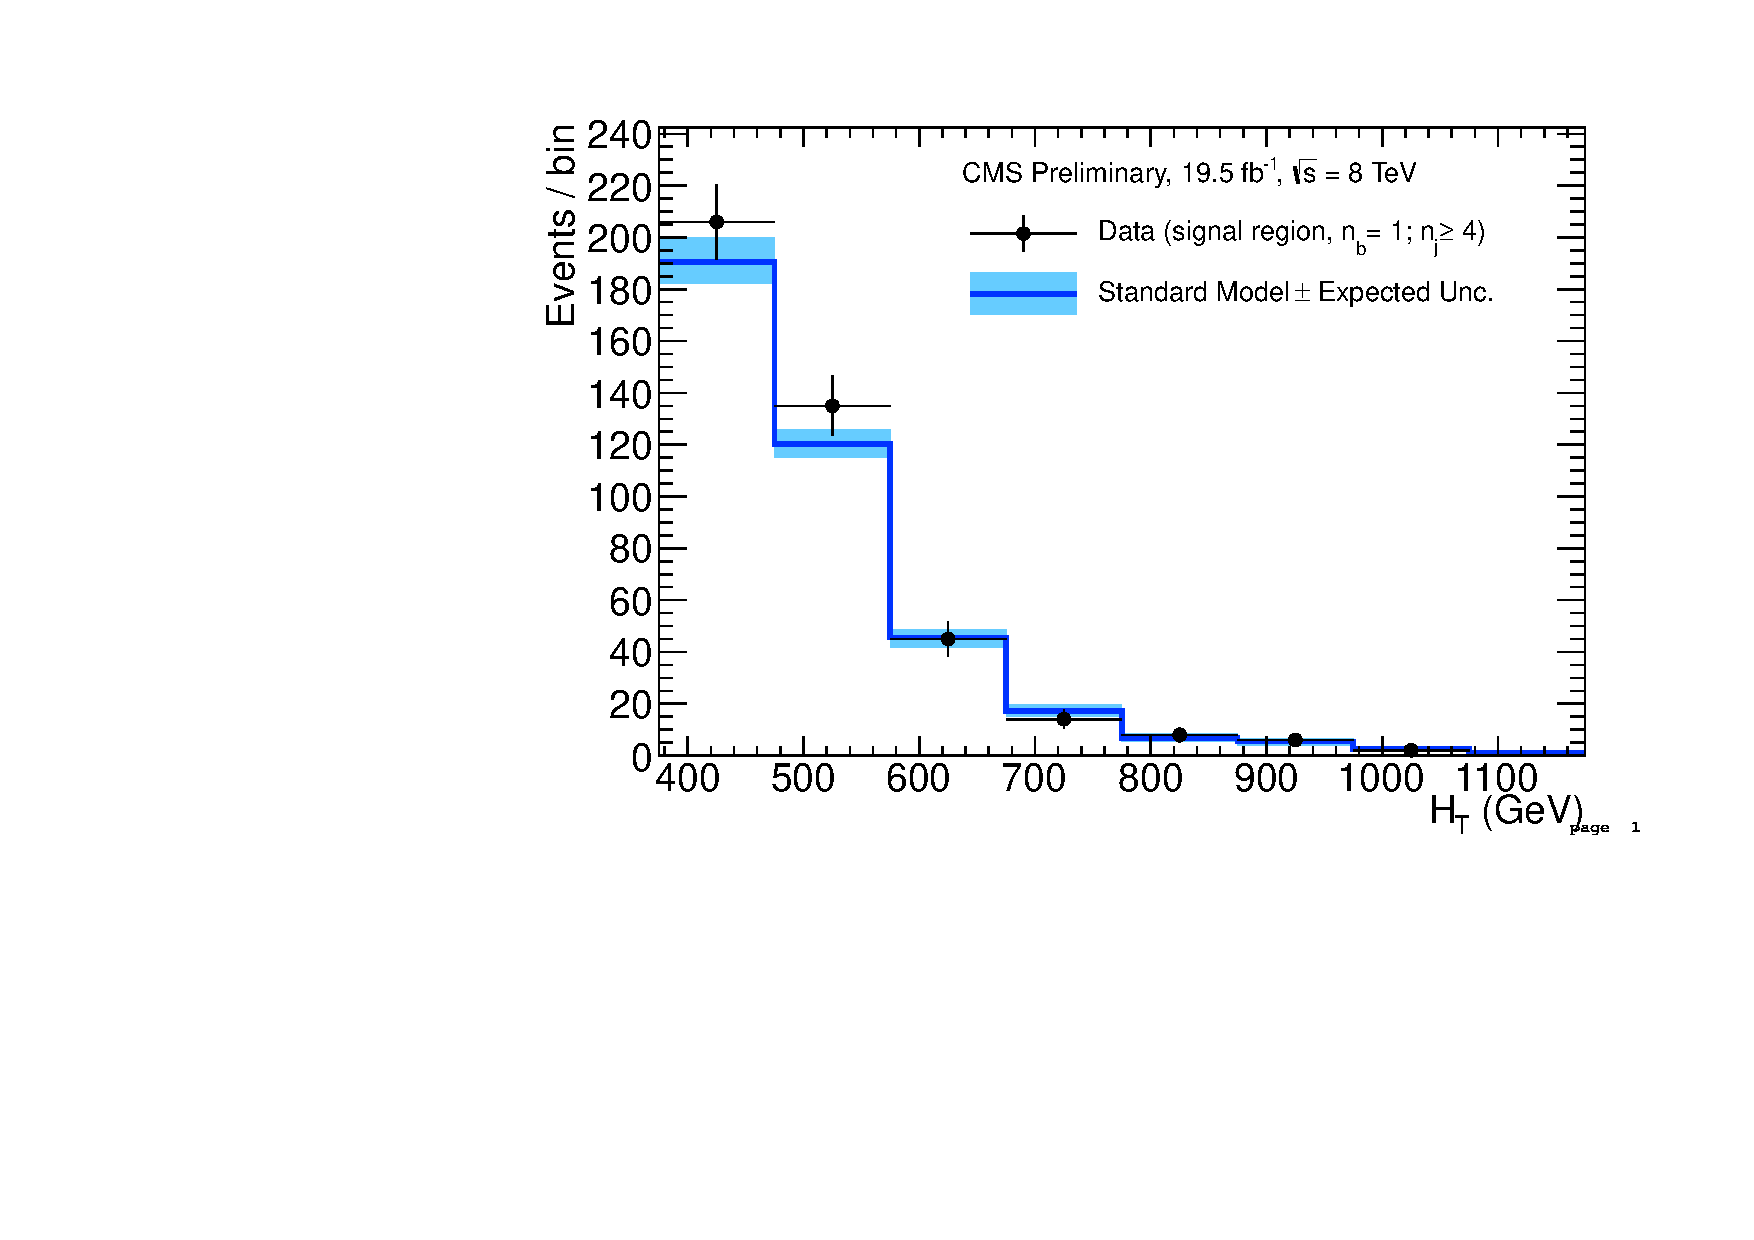
\includegraphics[width=0.45\textwidth,page=1]{figures/fit/v22/bestFit_2012pf_RQcdZero_fZinvAll_1b_ge4j-1hp_smOnly}
    } 
    \subfigure[Hadronic sample (logarithmic scale)]{
      \includegraphics[width=0.45\textwidth,page=2]{figures/fit/v22/bestFit_2012pf_RQcdZero_fZinvAll_1b_ge4j-1hp_smOnly}
    } \\
    \subfigure[$\mu$ + jets sample]{
      \includegraphics[width=0.45\textwidth,page=4]{figures/fit/v22/bestFit_2012pf_RQcdZero_fZinvAll_1b_ge4j-1hp_smOnly}
    } 
    \subfigure[$\gamma$ + jets sample]{
      \includegraphics[width=0.45\textwidth,page=6]{figures/fit/v22/bestFit_2012pf_RQcdZero_fZinvAll_1b_ge4j-1hp_smOnly}
    } 
    \caption{\label{fig:best-fit-ge4j1b} Comparison of the
      \scalht-binned observed data yields and SM expectations when
      requiring \njethigh and $\nb = 1$ for the (a-b) hadronic, (c)
      \mj, (d) \mmj and (e) \gj samples, as determined by a
      simultaneous fit to all data samples under the SM-only
      hypothesis. The observed event yields in data (black dots) and
      the expectations and their uncertainties (dark blue solid line
      with light blue bands), as determined by the simultaneous fit,
      are shown. 
      %For illustrative purposes only, the signal
      %expectations (pink dashed line) for the model \texttt{T2cc} with
      %$m_{\sq} = 250\GeV$ and $m_{\text{LSP}} = 170\GeV$ are stacked
      %on top of the SM expectations.
      }
  \end{center}
\end{figure}

\clearpage
\begin{figure}[t!]
  \begin{center}
    \subfigure[Hadronic sample (linear scale)]{
      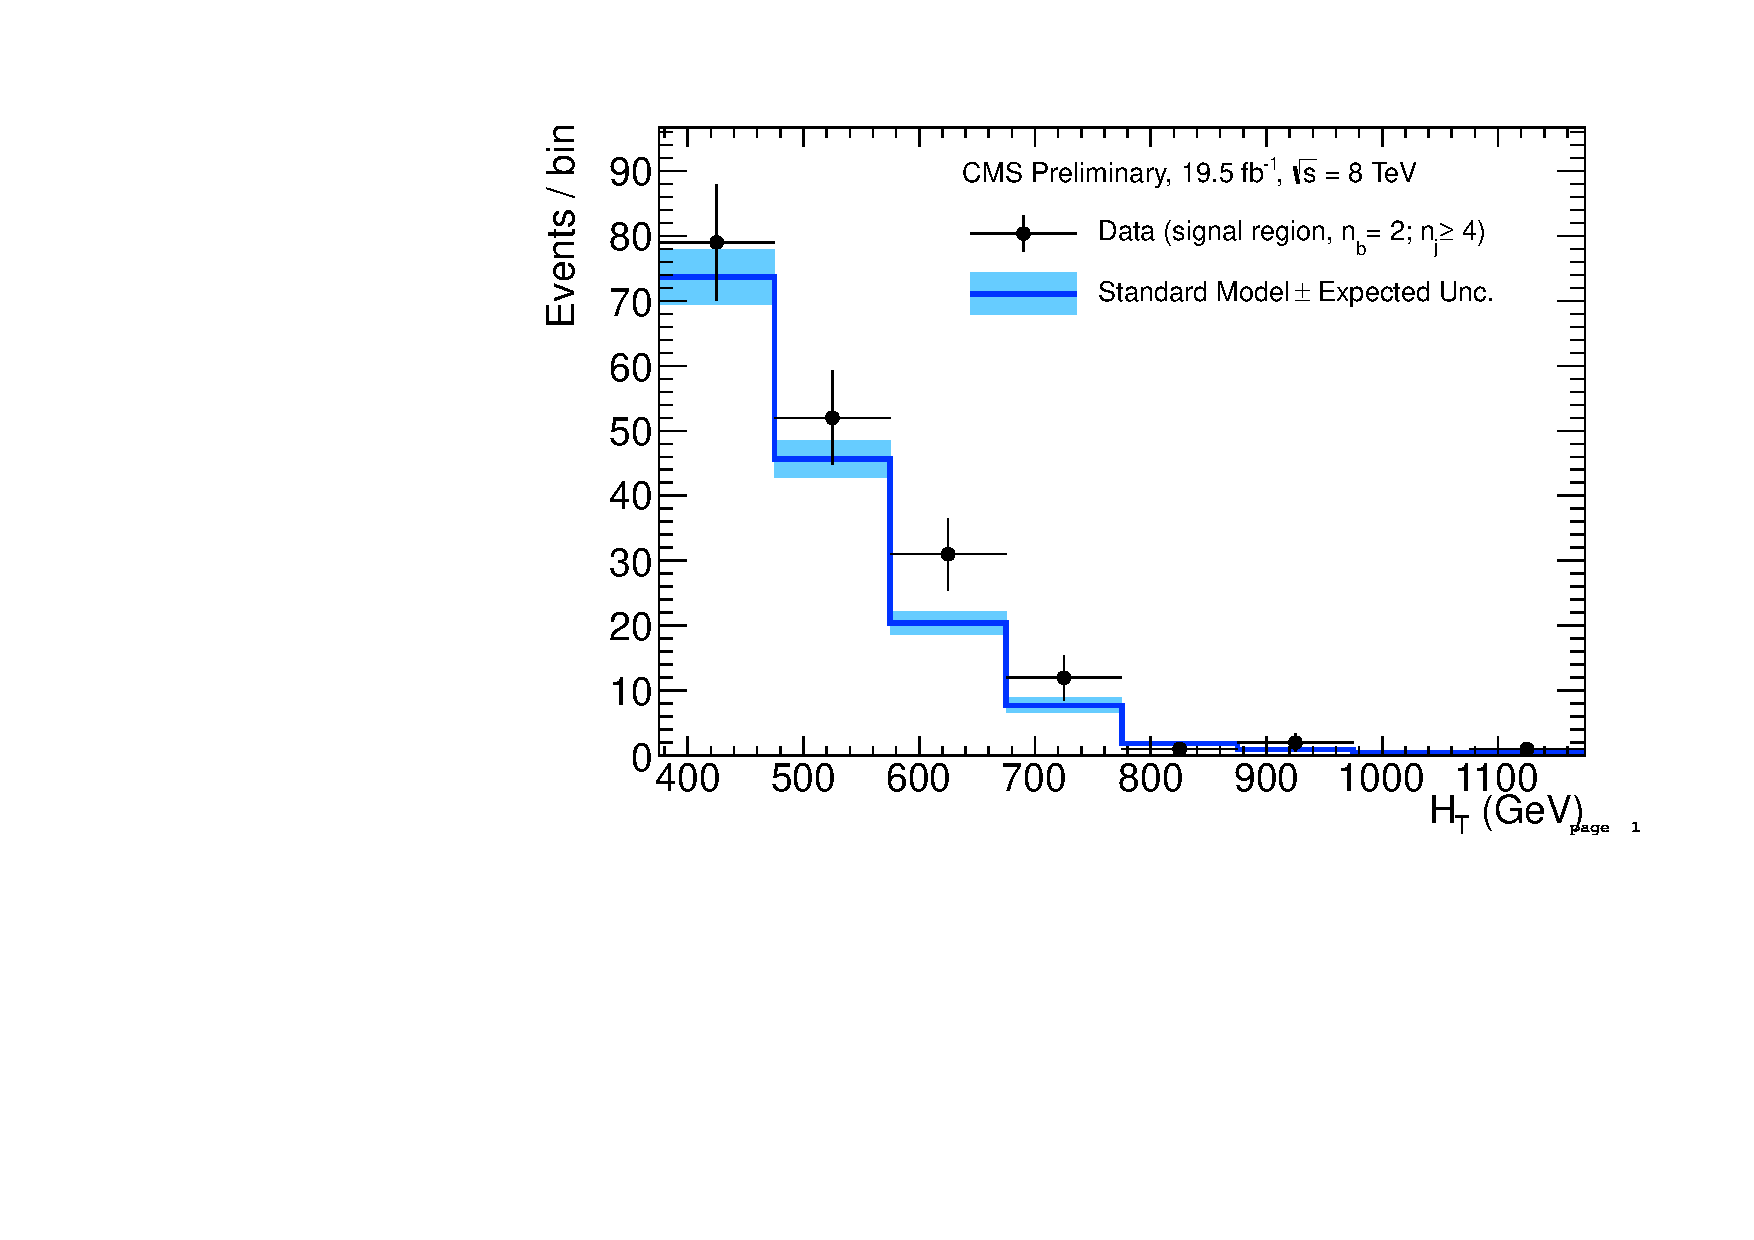
\includegraphics[width=0.45\textwidth,page=1]{figures/fit/v22/bestFit_2012pf_RQcdZero_fZinvAll_2b_ge4j-1h_smOnly}
    } 
    \subfigure[Hadronic sample (logarithmic scale)]{
      \includegraphics[width=0.45\textwidth,page=2]{figures/fit/v22/bestFit_2012pf_RQcdZero_fZinvAll_2b_ge4j-1h_smOnly}
    } \\
    \subfigure[$\mu$ + jets sample]{
      \includegraphics[width=0.45\textwidth,page=4]{figures/fit/v22/bestFit_2012pf_RQcdZero_fZinvAll_2b_ge4j-1h_smOnly}
    } 
    \caption{\label{fig:best-fit-ge4j2b} Comparison of the
      \scalht-binned observed data yields and SM expectations when
      requiring \njethigh and $\nb = 2$ for the (a-b) hadronic and \mj
      samples, as determined by a simultaneous fit to both the
      hadronic and \mj data samples under the SM-only hypothesis. The
      observed event yields in data (black dots) and the expectations
      and their uncertainties (dark blue solid line with light blue
      bands), as determined by the simultaneous fit, are shown. }
%      For illustrative purposes only, the signal expectations (pink
%      dashed line) for the model \texttt{T2cc} with $m_{\sq} =
%      250\GeV$ and $m_{\text{LSP}} = 240\GeV$ are stacked on top of
%      the SM expectations.}
  \end{center}
\end{figure}
%
%
%\clearpage
%\begin{figure}[t!]
%  \begin{center}
%    \subfigure[Hadronic sample (linear scale)]{
%      \includegraphics[width=0.45\textwidth,page=1]{figures/fit/v22/bestFit_2012pf_RQcdZero_fZinvAll_3b_ge4j-1h_smOnly}
%    } 
%    \subfigure[Hadronic sample (logarithmic scale)]{
%      \includegraphics[width=0.45\textwidth,page=2]{figures/fit/v22/bestFit_2012pf_RQcdZero_fZinvAll_3b_ge4j-1h_smOnly}
%    } \\
%    \subfigure[$\mu$ + jets sample]{
%      \includegraphics[width=0.45\textwidth,page=4]{figures/fit/v22/bestFit_2012pf_RQcdZero_fZinvAll_3b_ge4j-1h_smOnly}
%    } 
%    \caption{\label{fig:best-fit-ge4j3b} Comparison of the
%      \scalht-binned observed data yields and SM expectations when
%      requiring \njethigh and $\nb = 3$ for the (a-b) hadronic and \mj
%      samples, as determined by a simultaneous fit to both the
%      hadronic and \mj data samples under the SM-only hypothesis. The
%      observed event yields in data (black dots) and the expectations
%      and their uncertainties (dark blue solid line with light blue
%      bands), as determined by the simultaneous fit, are shown. }
%%      For illustrative purposes only, the signal expectations (pink
%%      dashed line) for the model \texttt{T2cc} with $m_{\sq} =
%%      250\GeV$ and $m_{\text{LSP}} = 240\GeV$ are stacked on top of
%%      the SM expectations.}
%  \end{center}
%\end{figure}
%
%
%\clearpage
%\begin{figure}[t!]
%  \begin{center}
%    \subfigure[Hadronic sample (linear scale)]{
%      \includegraphics[width=0.45\textwidth,page=1]{figures/fit/v22/bestFit_2012pf_RQcdZero_fZinvAll_ge4b_ge4j-1h_smOnly}
%    } 
%    \subfigure[Hadronic sample (logarithmic scale)]{
%      \includegraphics[width=0.45\textwidth,page=2]{figures/fit/v22/bestFit_2012pf_RQcdZero_fZinvAll_ge4b_ge4j-1h_smOnly}
%    } \\
%    \subfigure[$\mu$ + jets sample]{
%      \includegraphics[width=0.45\textwidth,page=4]{figures/fit/v22/bestFit_2012pf_RQcdZero_fZinvAll_ge4b_ge4j-1h_smOnly}
%    } 
%    \caption{\label{fig:best-fit-ge4jge4b} Comparison of the
%      \scalht-binned observed data yields and SM expectations when
%      requiring \njethigh and $\nb \geq 4$ for the (a-b) hadronic and \mj
%      samples, as determined by a simultaneous fit to both the
%      hadronic and \mj data samples under the SM-only hypothesis. The
%      observed event yields in data (black dots) and the expectations
%      and their uncertainties (dark blue solid line with light blue
%      bands), as determined by the simultaneous fit, are shown. }
%%      For illustrative purposes only, the signal expectations (pink
%%      dashed line) for the model \texttt{T2cc} with $m_{\sq} =
%%      250\GeV$ and $m_{\text{LSP}} = 240\GeV$ are stacked on top of
%%      the SM expectations.}
%  \end{center}
%\end{figure}

%\clearpage
\begin{figure}[t!]
  \begin{center}
    \subfigure[Hadronic sample (linear scale)]{
      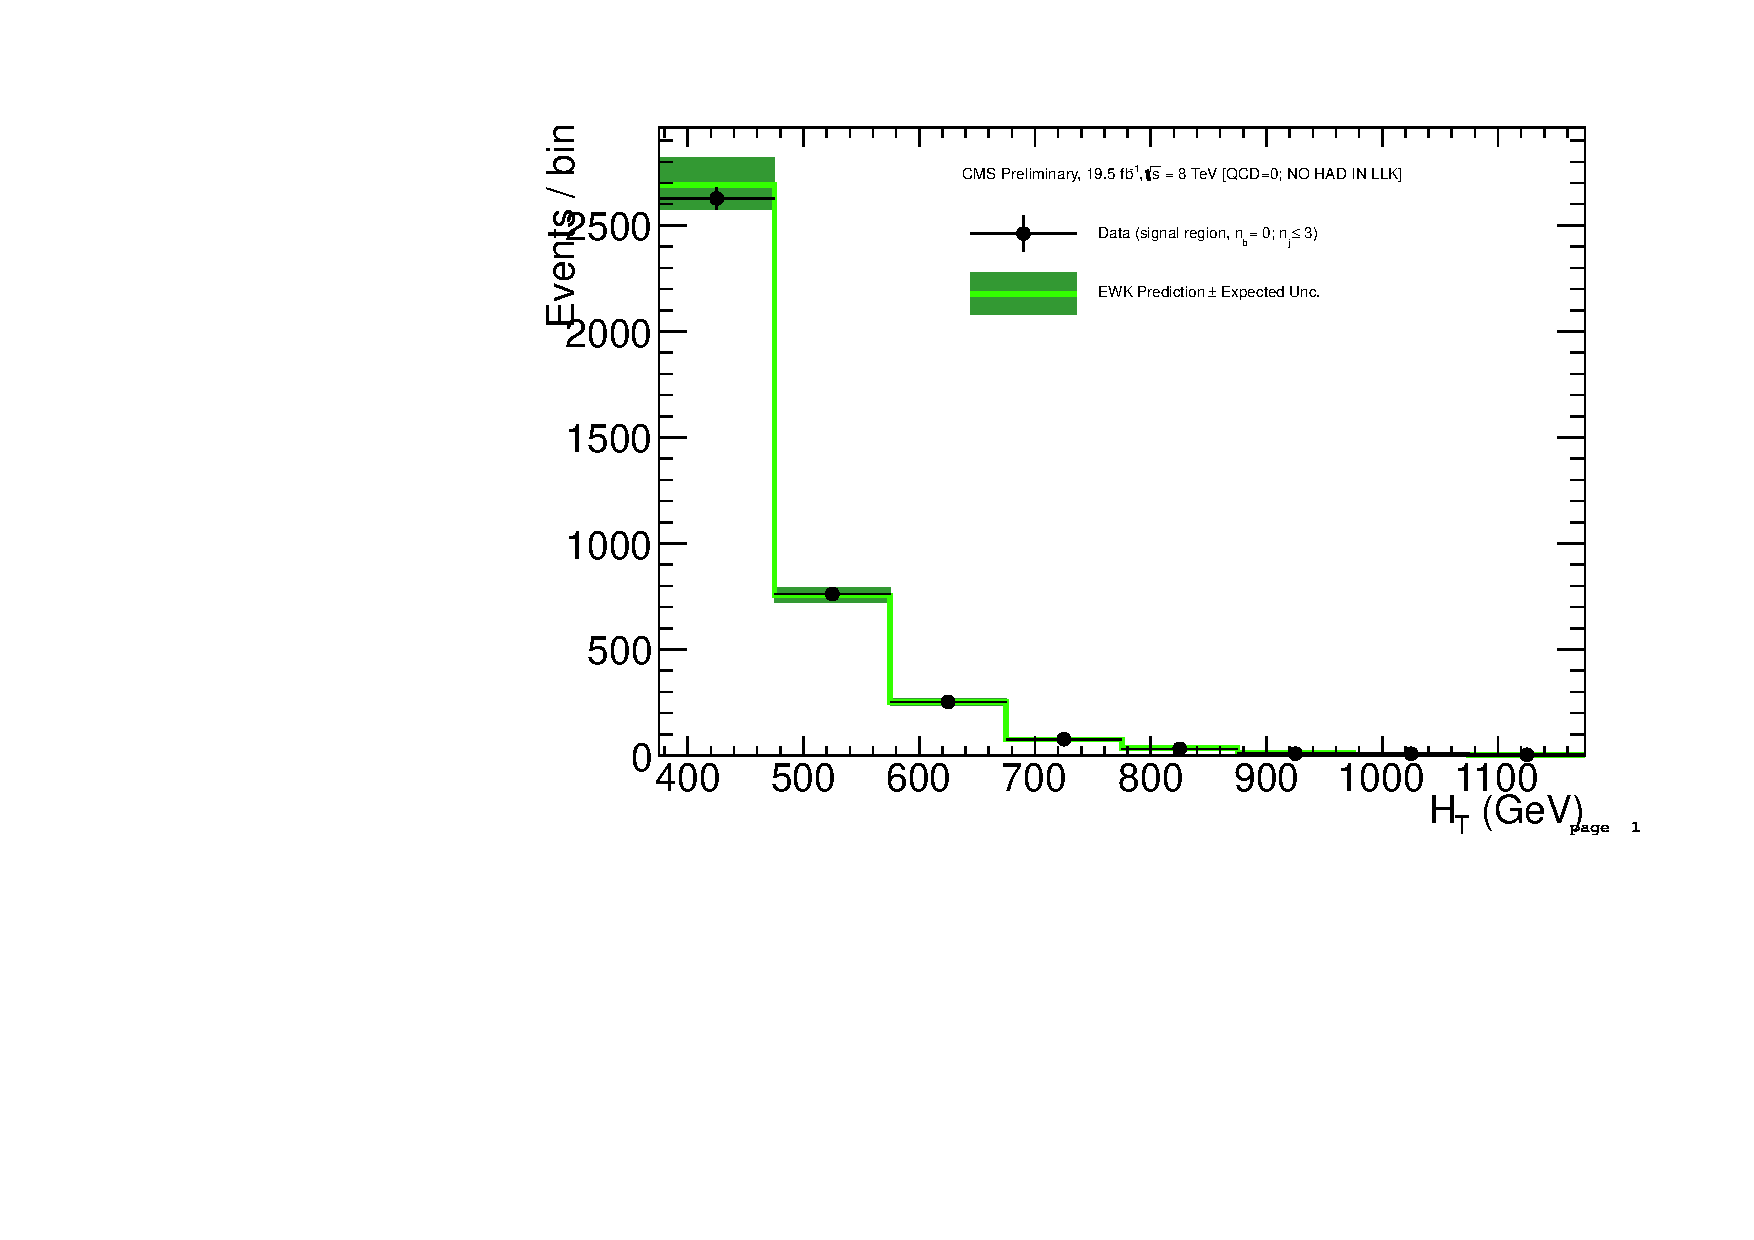
\includegraphics[width=0.45\textwidth,page=1]{figures/fit/v21/bestFit_2012pf_RQcdZero_fZinvAll_0b_le3j-1p_smOnly}
    } 
    \subfigure[Hadronic sample (logarithmic scale)]{
      \includegraphics[width=0.45\textwidth,page=2]{figures/fit/v21/bestFit_2012pf_RQcdZero_fZinvAll_0b_le3j-1p_smOnly}
    } \\
    \subfigure[$\mu$ + jets sample]{
      \includegraphics[width=0.45\textwidth,page=4]{figures/fit/v21/bestFit_2012pf_RQcdZero_fZinvAll_0b_le3j-1p_smOnly}
    } 
    \subfigure[$\gamma$ + jets sample]{
      \includegraphics[width=0.45\textwidth,page=6]{figures/fit/v21/bestFit_2012pf_RQcdZero_fZinvAll_0b_le3j-1p_smOnly}
    } 
    \caption{\label{fig:best-fit-control-only-le3j0b} Comparison of the
      \scalht-binned observed data yields and SM expectations
      when requiring \njetlow and $\nb = 0$ for the (a-b) hadronic,
      (c) \mj, (d) \mmj and (e) \gj samples, as determined by a
      simultaneous fit to the data control samples only. The observed
      event yields in data (black dots) and the expectations and their
      uncertainties (dark green solid line with light green bands), as
      determined by the simultaneous fit, are shown. }
%      For illustrative purposes only, the signal expectations (pink
%      dashed line) for the model \texttt{T2cc} with $m_{\sq} =
%      250\GeV$ and $m_{\text{LSP}} = 240\GeV$ are stacked on top of
%      the SM expectations.}
  \end{center}
\end{figure}

\clearpage
\begin{figure}[t!]
  \begin{center}
    \subfigure[Hadronic sample (linear scale)]{
      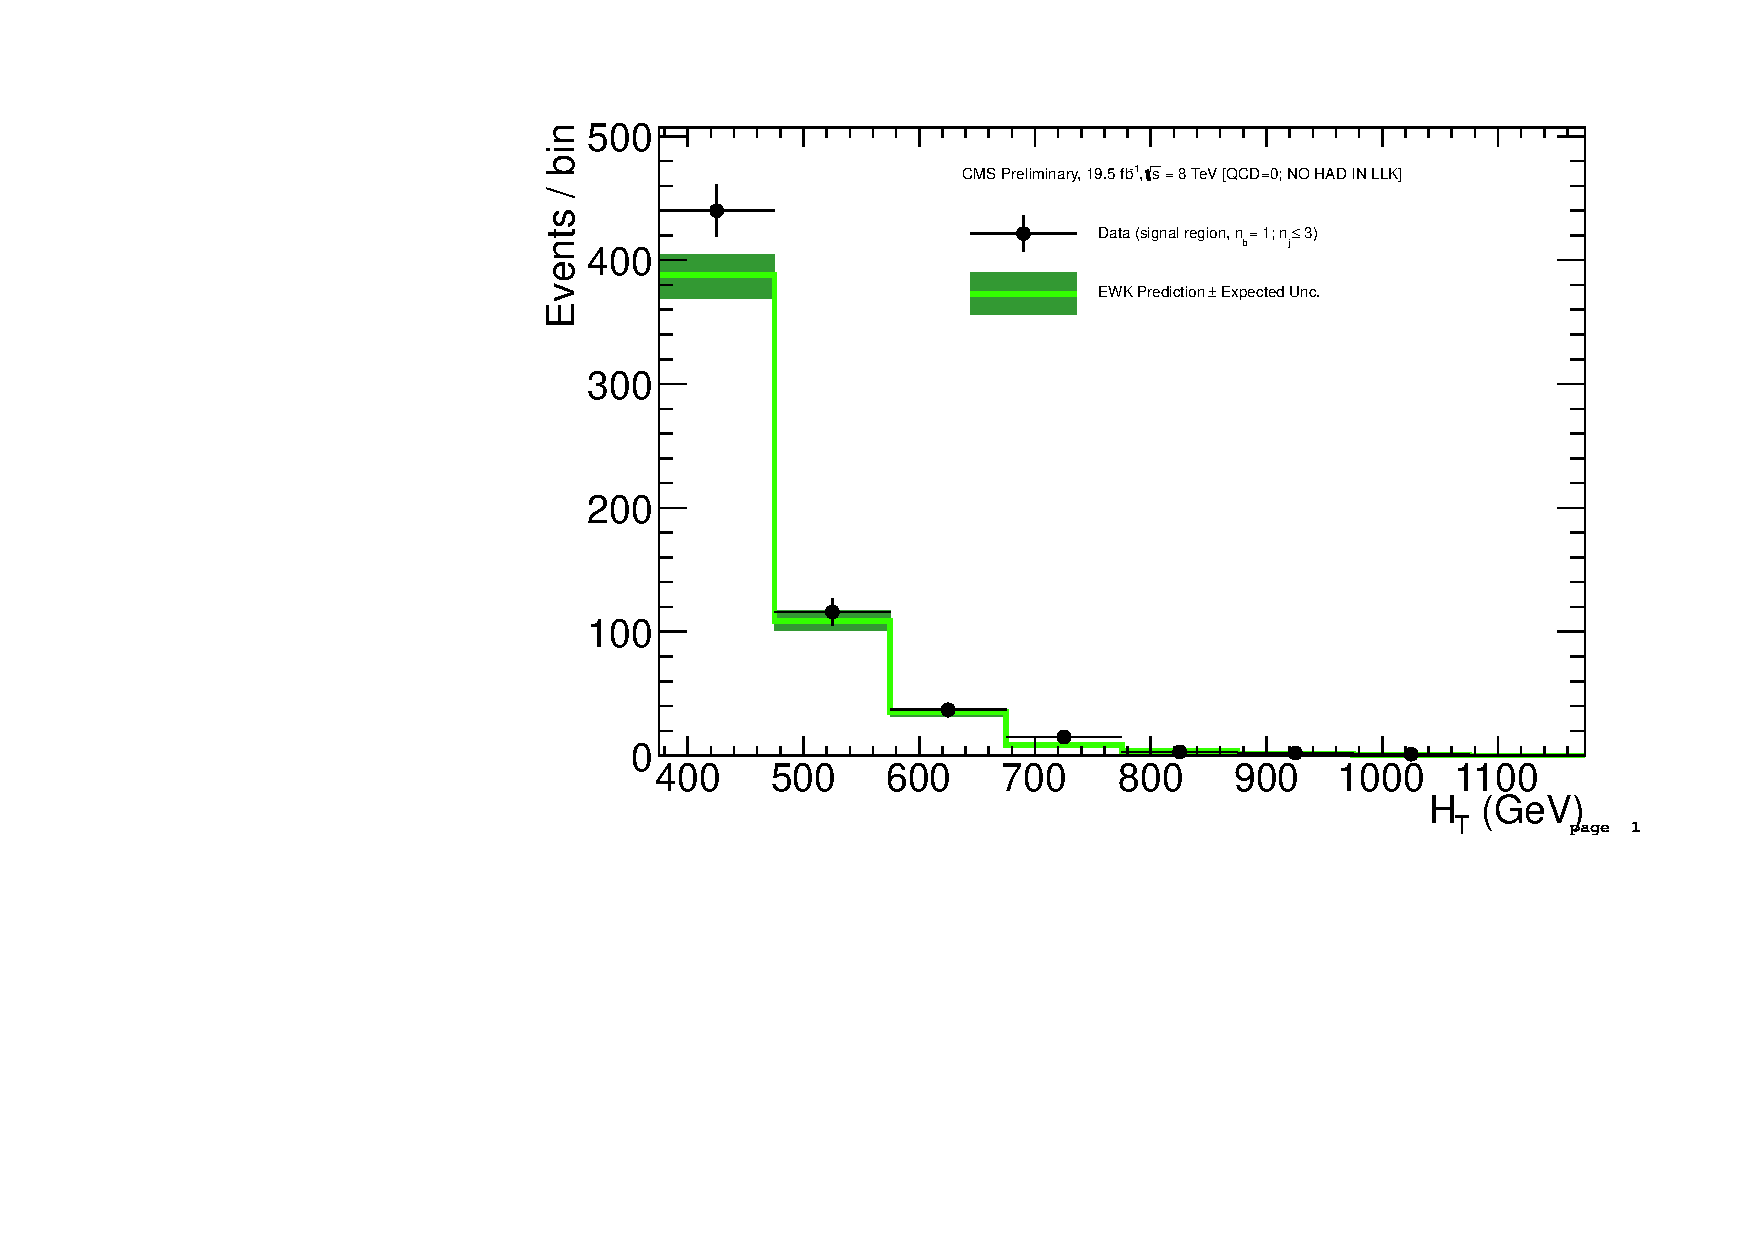
\includegraphics[width=0.45\textwidth,page=1]{figures/fit/v21/bestFit_2012pf_RQcdZero_fZinvAll_1b_le3j-1p_smOnly}
    } 
    \subfigure[Hadronic sample (logarithmic scale)]{
      \includegraphics[width=0.45\textwidth,page=2]{figures/fit/v21/bestFit_2012pf_RQcdZero_fZinvAll_1b_le3j-1p_smOnly}
    } \\
    \subfigure[$\mu$ + jets sample]{
      \includegraphics[width=0.45\textwidth,page=4]{figures/fit/v21/bestFit_2012pf_RQcdZero_fZinvAll_1b_le3j-1p_smOnly}
    } 
    \subfigure[$\gamma$ + jets sample]{
      \includegraphics[width=0.45\textwidth,page=6]{figures/fit/v21/bestFit_2012pf_RQcdZero_fZinvAll_1b_le3j-1p_smOnly}
    } 
    \caption{\label{fig:best-fit-control-only-le3j1b} Comparison of the
      \scalht-binned observed data yields and SM expectations when
      requiring \njetlow and $\nb = 1$ for the (a-b) hadronic, (c)
      \mj, (d) \mmj and (e) \gj samples, as determined by a
      simultaneous fit to the data control samples only. The observed
      event yields in data (black dots) and the expectations and their
      uncertainties (dark green solid line with light green bands), as
      determined by the simultaneous fit, are shown. }
%      For illustrative purposes only, the signal expectations (pink
%      dashed line) for the model \texttt{T2cc} with $m_{\sq} =
%      250\GeV$ and $m_{\text{LSP}} = 170\GeV$ are stacked on top of
%      the SM expectations.}
  \end{center}
\end{figure}

\clearpage
\begin{figure}[t!]
  \begin{center}
    \subfigure[Hadronic sample (linear scale)]{
      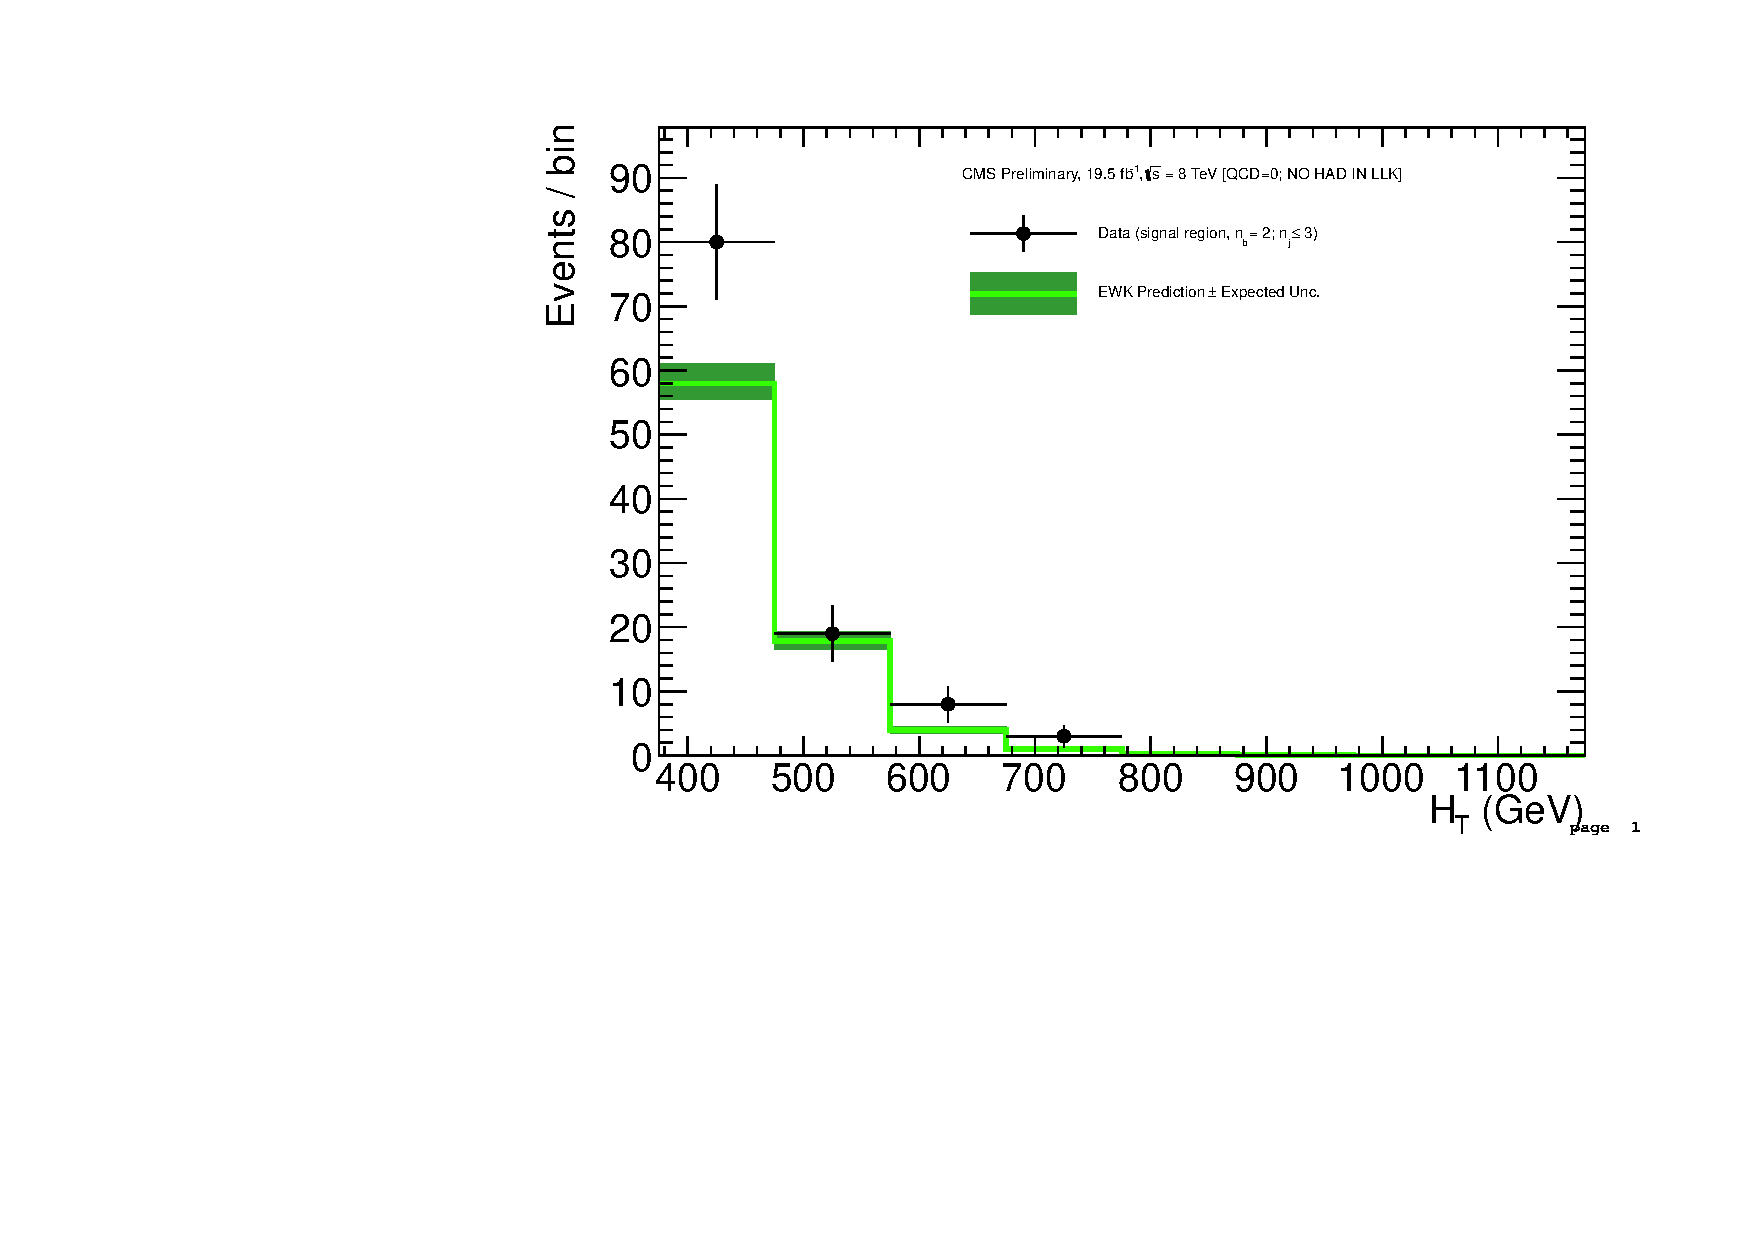
\includegraphics[width=0.45\textwidth,page=1]{figures/fit/v21/bestFit_2012pf_RQcdZero_fZinvAll_2b_le3j-1_smOnly}
    } 
    \subfigure[Hadronic sample (logarithmic scale)]{
      \includegraphics[width=0.45\textwidth,page=2]{figures/fit/v21/bestFit_2012pf_RQcdZero_fZinvAll_2b_le3j-1_smOnly}
    } \\
    \subfigure[$\mu$ + jets sample]{
      \includegraphics[width=0.45\textwidth,page=4]{figures/fit/v21/bestFit_2012pf_RQcdZero_fZinvAll_2b_le3j-1_smOnly}
    } 
    \caption{\label{fig:best-fit-control-only-le3j2b} Comparison of the
      \scalht-binned observed data yields and SM expectations when
      requiring \njetlow and $\nb = 2$ for the (a-b) hadronic, (c)
      \mj, (d) \mmj and (e) \gj samples, as determined by the \mj data
      control sample only. The observed event yields in data (black
      dots) and the expectations and their uncertainties (dark green
      solid line with light green bands) are shown. }
%      For illustrative purposes only, the signal expectations (pink
%      dashed line) for the model \texttt{T2cc} with $m_{\sq} =
%      250\GeV$ and $m_{\text{LSP}} = 240\GeV$ are stacked on top of
%      the SM expectations.}
  \end{center}
\end{figure}

\clearpage
\begin{figure}[t!]
  \begin{center}
    \subfigure[Hadronic sample (linear scale)]{
      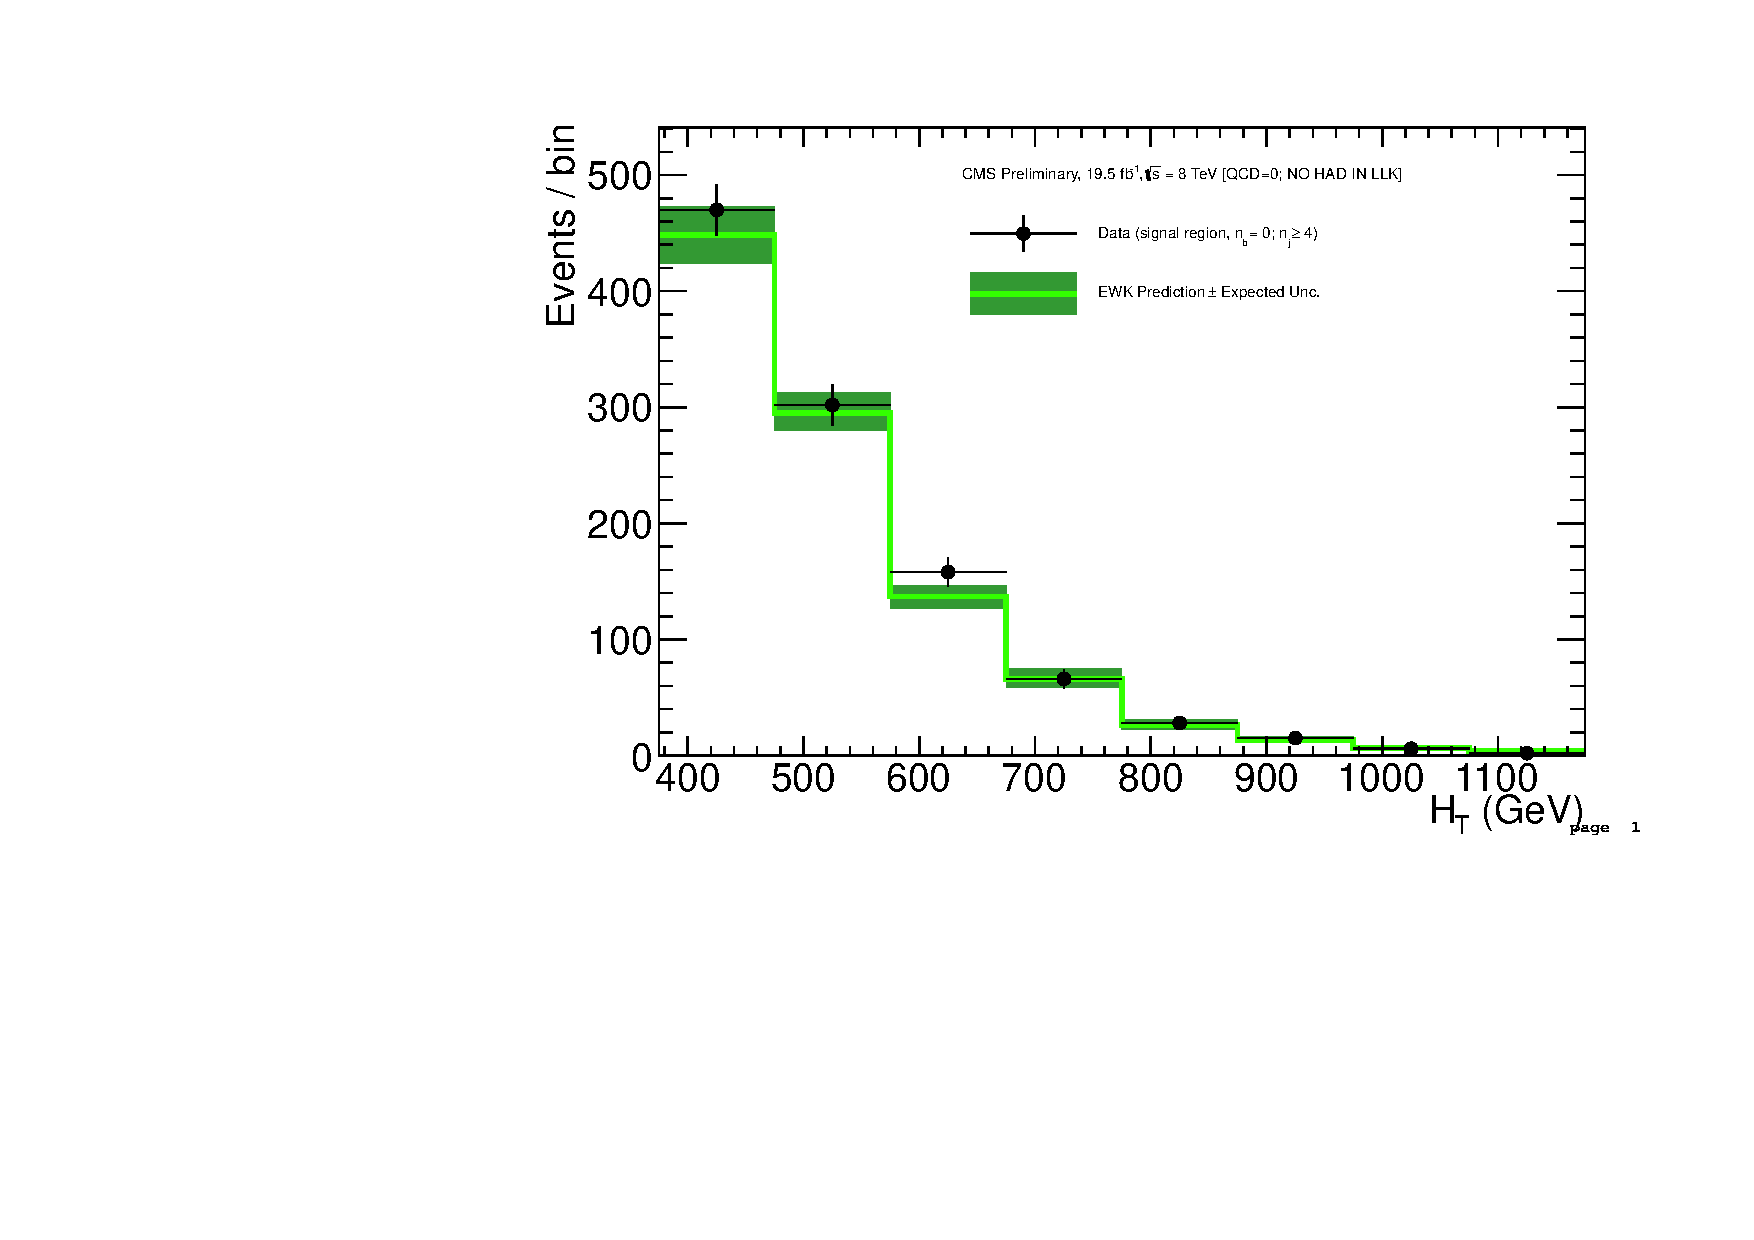
\includegraphics[width=0.45\textwidth,page=1]{figures/fit/v21/bestFit_2012pf_RQcdZero_fZinvAll_0b_ge4j-1p_smOnly}
    } 
    \subfigure[Hadronic sample (logarithmic scale)]{
      \includegraphics[width=0.45\textwidth,page=2]{figures/fit/v21/bestFit_2012pf_RQcdZero_fZinvAll_0b_ge4j-1p_smOnly}
    } \\
    \subfigure[$\mu$ + jets sample]{
      \includegraphics[width=0.45\textwidth,page=4]{figures/fit/v21/bestFit_2012pf_RQcdZero_fZinvAll_0b_ge4j-1p_smOnly}
    } 
    \subfigure[$\gamma$ + jets sample]{
      \includegraphics[width=0.45\textwidth,page=6]{figures/fit/v21/bestFit_2012pf_RQcdZero_fZinvAll_0b_ge4j-1p_smOnly}
    } 
    \caption{\label{fig:best-fit-control-only-ge4j0b} Comparison of the
      \scalht-binned observed data yields and SM expectations when
      requiring \njethigh and $\nb = 0$ for the (a-b) hadronic, (c)
      \mj, (d) \mmj and (e) \gj samples, as determined by a
      simultaneous fit to the data control samples only. The observed
      event yields in data (black dots) and the expectations and their
      uncertainties (dark green solid line with light green bands), as
      determined by the simultaneous fit, are shown. }
%      For illustrative purposes only, the signal expectations (pink
%      dashed line) for the model \texttt{T2cc} with $m_{\sq} =
%      250\GeV$ and $m_{\text{LSP}} = 170\GeV$ are stacked on top of
%      the SM expectations.}
  \end{center}
\end{figure}

\clearpage
\begin{figure}[t!]
  \begin{center}
    \subfigure[Hadronic sample (linear scale)]{
      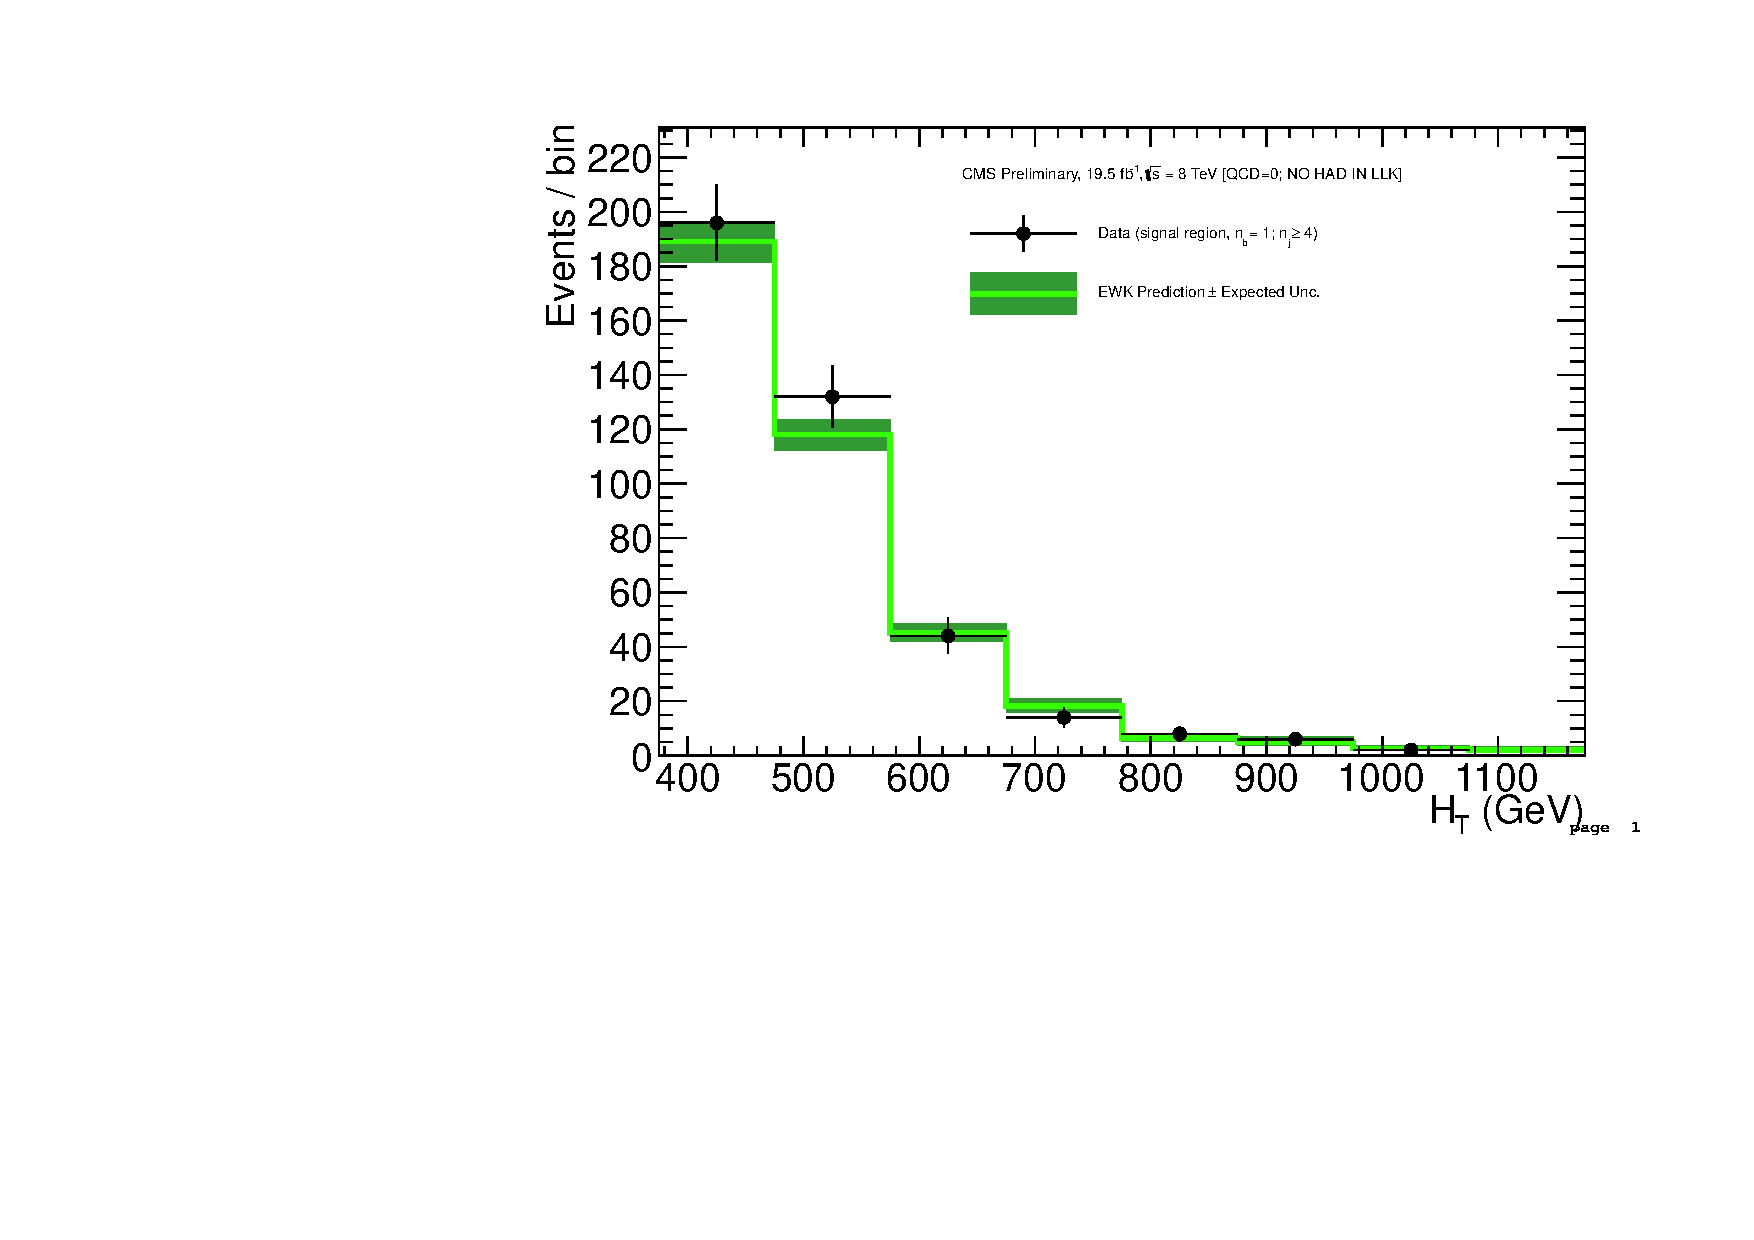
\includegraphics[width=0.45\textwidth,page=1]{figures/fit/v21/bestFit_2012pf_RQcdZero_fZinvAll_1b_ge4j-1p_smOnly}
    } 
    \subfigure[Hadronic sample (logarithmic scale)]{
      \includegraphics[width=0.45\textwidth,page=2]{figures/fit/v21/bestFit_2012pf_RQcdZero_fZinvAll_1b_ge4j-1p_smOnly}
    } \\
    \subfigure[$\mu$ + jets sample]{
      \includegraphics[width=0.45\textwidth,page=4]{figures/fit/v21/bestFit_2012pf_RQcdZero_fZinvAll_1b_ge4j-1p_smOnly}
    } 
    \subfigure[$\gamma$ + jets sample]{
      \includegraphics[width=0.45\textwidth,page=6]{figures/fit/v21/bestFit_2012pf_RQcdZero_fZinvAll_1b_ge4j-1p_smOnly}
    } 
    \caption{\label{fig:best-fit-control-only-ge4j1b} Comparison of the
      \scalht-binned observed data yields and SM expectations when
      requiring \njethigh and $\nb = 1$ for the (a-b) hadronic, (c)
      \mj, (d) \mmj and (e) \gj samples, as determined by a
      simultaneous fit to the data control samples only. The observed
      event yields in data (black dots) and the expectations and their
      uncertainties (dark green solid line with light green bands), as
      determined by the simultaneous fit, are shown. }
%      For illustrative purposes only, the signal expectations (pink
%      dashed line) for the model \texttt{T2cc} with $m_{\sq} =
%      250\GeV$ and $m_{\text{LSP}} = 170\GeV$ are stacked on top of
%      the SM expectations.}
  \end{center}
\end{figure}

\clearpage
\begin{figure}[t!]
  \begin{center}
    \subfigure[Hadronic sample (linear scale)]{
      \includegraphics[width=0.45\textwidth,page=1]{figures/fit/v21/bestFit_2012pf_RQcdZero_fZinvAll_2b_ge4j-1_smOnly}
    } 
    \subfigure[Hadronic sample (logarithmic scale)]{
      \includegraphics[width=0.45\textwidth,page=2]{figures/fit/v21/bestFit_2012pf_RQcdZero_fZinvAll_2b_ge4j-1_smOnly}
    } \\
    \subfigure[$\mu$ + jets sample]{
      \includegraphics[width=0.45\textwidth,page=4]{figures/fit/v21/bestFit_2012pf_RQcdZero_fZinvAll_2b_ge4j-1_smOnly}
    } 
    \caption{\label{fig:best-fit-control-only-ge4j2b} Comparison of the
      \scalht-binned observed data yields and SM expectations when
      requiring \njethigh and $\nb = 2$ for the (a-b) hadronic, (c)
      \mj, (d) \mmj and (e) \gj samples, as determined by the \mj data
      control sample only. The observed event yields in data (black
      dots) and the expectations and their uncertainties (dark green
      solid line with light green bands) are shown. }
%      For illustrative purposes only, the signal expectations (pink
%      dashed line) for the model \texttt{T2cc} with $m_{\sq} =
%      250\GeV$ and $m_{\text{LSP}} = 240\GeV$ are stacked on top of
%      the SM expectations.}
  \end{center}
\end{figure}


%\clearpage
%\begin{figure}[t!]
%  \begin{center}
%    \subfigure[Hadronic sample (linear scale)]{
%      \includegraphics[width=0.45\textwidth,page=1]{figures/fit/v21/bestFit_2012pf_RQcdZero_fZinvAll_3b_ge4j-1_smOnly}
%    } 
%    \subfigure[Hadronic sample (logarithmic scale)]{
%      \includegraphics[width=0.45\textwidth,page=2]{figures/fit/v21/bestFit_2012pf_RQcdZero_fZinvAll_3b_ge4j-1_smOnly}
%    } \\
%    \subfigure[$\mu$ + jets sample]{
%      \includegraphics[width=0.45\textwidth,page=4]{figures/fit/v21/bestFit_2012pf_RQcdZero_fZinvAll_3b_ge4j-1_smOnly}
%    } 
%    \caption{\label{fig:best-fit-control-only-ge4j3b} Comparison of the
%      \scalht-binned observed data yields and SM expectations when
%      requiring \njethigh and $\nb = 3$ for the (a-b) hadronic, (c)
%      \mj, (d) \mmj and (e) \gj samples, as determined by the \mj data
%      control sample only. The observed event yields in data (black
%      dots) and the expectations and their uncertainties (dark green
%      solid line with light green bands) are shown. }
%%      For illustrative purposes only, the signal expectations (pink
%%      dashed line) for the model \texttt{T2cc} with $m_{\sq} =
%%      250\GeV$ and $m_{\text{LSP}} = 240\GeV$ are stacked on top of
%%      the SM expectations.}
%  \end{center}
%\end{figure}
%
%
%\clearpage
%\begin{figure}[t!]
%  \begin{center}
%    \subfigure[Hadronic sample (linear scale)]{
%      \includegraphics[width=0.45\textwidth,page=1]{figures/fit/v21/bestFit_2012pf_RQcdZero_fZinvAll_ge4b_ge4j-1_smOnly}
%    } 
%    \subfigure[Hadronic sample (logarithmic scale)]{
%      \includegraphics[width=0.45\textwidth,page=2]{figures/fit/v21/bestFit_2012pf_RQcdZero_fZinvAll_ge4b_ge4j-1_smOnly}
%    } \\
%    \subfigure[$\mu$ + jets sample]{
%      \includegraphics[width=0.45\textwidth,page=4]{figures/fit/v21/bestFit_2012pf_RQcdZero_fZinvAll_ge4b_ge4j-1_smOnly}
%    } 
%    \caption{\label{fig:best-fit-control-only-ge4jge4b} Comparison of the
%      \scalht-binned observed data yields and SM expectations when
%      requiring \njethigh and $\nb \geq 4$ for the (a-b) hadronic, (c)
%      \mj, (d) \mmj and (e) \gj samples, as determined by the \mj data
%      control sample only. The observed event yields in data (black
%      dots) and the expectations and their uncertainties (dark green
%      solid line with light green bands) are shown. }
%%      For illustrative purposes only, the signal expectations (pink
%%      dashed line) for the model \texttt{T2cc} with $m_{\sq} =
%%      250\GeV$ and $m_{\text{LSP}} = 240\GeV$ are stacked on top of
%%      the SM expectations.}
%  \end{center}
%\end{figure}

